\documentclass[11pt,a4paper]{article}
\usepackage[T1]{fontenc}
\usepackage[utf8]{inputenc}
\usepackage[brazil]{babel}
\usepackage{lmodern}
\usepackage{amsmath,amssymb,bm,mathtools}
\usepackage{geometry}
\usepackage{booktabs,array,longtable,multirow}
\usepackage{graphicx}
\usepackage[ruled,lined,linesnumbered,portuguese]{algorithm2e}
\usepackage{hyperref}
\geometry{margin=2.3cm}
\setlength{\parindent}{0pt}
\setlength{\parskip}{5pt}
\numberwithin{equation}{section}
\allowdisplaybreaks
\renewcommand{\arraystretch}{1.05}
\hypersetup{colorlinks=true,linkcolor=black,citecolor=black,urlcolor=black}
\renewcommand{\topfraction}{0.9}
\renewcommand{\bottomfraction}{0.8}
\renewcommand{\textfraction}{0.1}
\renewcommand{\floatpagefraction}{0.8}
\emergencystretch=2em
\SetKwIF{If}{ElseIf}{Else}{se}{então}{senão, se}{senão}{fim}
\SetKwFor{For}{para}{faça}{fim}
\SetKwRepeat{Repeat}{repita}{até}
\SetKwProg{Fn}{função}{}{fim}
\SetKw{Return}{retornar}

\title{Cálculo do fator de segurança de um talude não saturado sob chuva:\\
SRM e GIM, com e sem arc-length\\[3pt]
\large Formulação, análise de sensibilidade e parâmetros recomendados}
\author{}
\date{7 de novembro de 2026}


\begin{document}

\maketitle

\vspace{-1.5em}

\begin{abstract}
Este relatório compara o cálculo do fator de segurança (FS) de um talude não saturado sob chuva, baseado em Rahardjo et al.\ (2007), pelos métodos de redução de resistência (SRM) e de aumento da gravidade (GIM), com lista e bisseção e com arc-length. A análise de sensibilidade usou mais de 1600 rodadas, em 43 casos. A configuração final do arc-length gasta 35\% menos iterações de Newton que o SRM antigo (cerca de 22\% menos de tempo, por estimativa), com pior erro de $-0{,}46\%$ em relação à referência, contra $-1{,}11\%$. No GIM, o custo é parecido (7\% menos iterações), mas o pior erro cai de $-26{,}87\%$ para $-0{,}41\%$, e o resultado deixa de variar com o número de threads. Os parâmetros recomendados são: parada $\Delta\Lambda < 0{,}001$ medida no comprimento pedido, preditor secante com a superfície de escoamento levemente encolhida, $\alpha = 0{,}1$ sem lista no SRM, \texttt{alvo} = 10 e \texttt{maxIt} = 12, com \texttt{lMax} = 0,5 no SRM e 2 no GIM. A tolerância 0,01 não atende ao limite de erro de 1\% em vários casos. Os mesmos parâmetros, sem ajuste, foram depois aplicados ao modelo acoplado com ar ativo, no caso base: todos os cálculos pararam pelo critério, com pior erro de $-0{,}41\%$ no SRM e $-0{,}29\%$ no GIM.
\end{abstract}


\tableofcontents

\section{O problema}\label{sec:problema}

\subsection{Objetivo}

Rahardjo et al.~\cite{rahardjo2007} estudaram os fatores que controlam a instabilidade de taludes homogêneos de solo não saturado
sob chuva. A chuva reduz a sucção perto da superfície, a resistência cai e o fator de segurança (FS) diminui ao longo do
tempo; depois que a chuva termina, a água se redistribui e o FS volta a subir. O resultado de interesse é a curva FS$(t)$. No
artigo, ela é obtida com percolação em SEEP/W e equilíbrio limite (Bishop simplificado) em SLOPE/W. Aqui, o mesmo problema
é resolvido com elementos finitos elastoplásticos, em NeoPZ.

Cada ponto da curva exige um cálculo completo de FS, que é uma sequência de problemas não lineares. Um estudo de Monte Carlo com
campos aleatórios repete esse cálculo milhares de vezes. Por isso importam três coisas: o método precisa dar uma resposta em
todos os casos, a resposta precisa estar próxima do valor verdadeiro, e o custo precisa ser baixo. Este relatório compara, com
esses três critérios, os métodos de redução de resistência (SRM) e de aumento da gravidade (GIM), com e sem arc-length.

\subsection{Geometria e malha}

A Figura~\ref{fig:geometria} mostra o caso base: altura $H_s = 10$~m, inclinação $\beta = 45^\circ$, pé em $(40,\,20)$~m e crista em
$(30,\,30)$~m, com platôs de 30~m. O nível d'água inicial está $H_w = 5$~m abaixo do pé e tem inclinação de $7^\circ$:
$y_w(x) = 15 + (40 - x)\tan 7^\circ$. (O artigo chama a inclinação do talude de $\alpha$; aqui $\alpha$ fica reservado à restrição do
arc-length.)

\begin{figure}[htbp]
\centering
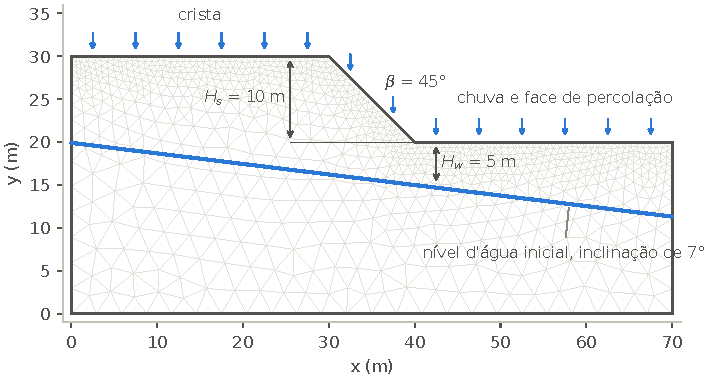
\includegraphics[width=\linewidth]{figuras/geometria.pdf}
\caption{Geometria e malha do caso base, com as condições de contorno hidráulicas.}\label{fig:geometria}
\end{figure}

A malha tem 1684 triângulos e 918 vértices, em estado plano de deformação, com tamanho de 0,75~m até 2~m de profundidade, crescendo
até 3~m. Os deslocamentos são quadráticos e as pressões são lineares, o que dá 8874 equações. Mecanicamente, a base é fixa e as
laterais têm $u_x = 0$.

\subsection{Parâmetros}

Os valores estão na Tabela~\ref{tab:parametros}. O nome do solo segue o artigo: f50,$-5$ significa parâmetro $a = 50$~kPa da curva de
retenção e condutividade saturada $k_s = 10^{-5}$~m/s. O artigo não informa $E$ e $\nu$, que são hipóteses deste estudo. Eles
influenciam os deslocamentos, mas não o limite de equilíbrio.

\begin{table}[htbp]
\centering\footnotesize
\caption{Parâmetros do caso base.}\label{tab:parametros}
\begin{tabular}{p{6.2cm}p{5.0cm}p{3.6cm}}
\toprule
Grandeza & Valor & Origem \\
\midrule
Coesão efetiva $c'$ & 10 kPa & artigo \\
Ângulo de atrito $\phi'$ & $26^\circ$ & artigo \\
Ângulo de dilatância $\psi$ & $\psi = \phi'$ (fluxo associado) & exigência da projeção analítica \\
Parcela de sucção & $\chi = 1$, ou seja, $\phi^b = \phi'$ & artigo \\
Peso específico $\gamma$ & 20 kN/m$^3$ & artigo \\
Módulo $E$, Poisson $\nu$ & 20 MPa; 0,3 & hipótese \\
Porosidade $n$ & 0,45 ($\theta_s$ do artigo) & artigo \\
Condutividade saturada $k_s$ & $10^{-5}$ m/s & artigo \\
Retenção (Fredlund--Xing) & $a = 50$ kPa, $n_{FX} = m_{FX} = 1$ & artigo \\
Permeabilidade relativa & $k_{rw} = S_w^{\,4}$ & artigo \\
Peso específico da água $\gamma_w$, compressibilidade $K_w$ & 9,81 kN/m$^3$; $2{,}2\times10^{6}$ kPa & código \\
Chuva & 36 mm/h durante 24 h & artigo \\
Transiente & 48 h, $\Delta t = 0{,}1$ h & código \\
\bottomrule
\end{tabular}
\end{table}

\subsection{Modelo}

As incógnitas são os deslocamentos $\mathbf{u}$ e as pressões $p_w$ e $p_a$. A tensão total é
\begin{equation}
\boldsymbol\sigma = \boldsymbol\sigma' - \alpha_B\, p_B\,\mathbf{I}, \qquad p_B = \chi\, p_w + (1-\chi)\, p_a,
\end{equation}
com coeficiente de Biot $\alpha_B = 1$ e tração positiva. A tensão efetiva $\boldsymbol\sigma'$ vem de um modelo de Mohr--Coulomb
elastoplástico perfeito, com projeção analítica e tangente consistente. Com $\chi = 1$ tem-se $p_B = p_w$, e a sucção contribui
para a resistência na mesma taxa que a tensão normal. O equilíbrio discreto é
\begin{equation}\label{eq:equilibrio}
\int_\Omega \mathbf{B}^{\mathsf T}\boldsymbol\sigma'(\mathbf{u})\,\mathrm{d}\Omega
- \alpha_B \int_\Omega \mathbf{m}\, p_B\,\mathrm{d}\Omega
- \int_\Omega \mathbf{N}^{\mathsf T}\gamma\,\mathbf{g}\,\mathrm{d}\Omega = \mathbf{0},
\end{equation}
em que $\mathbf{m}$ reúne a divergência das funções de forma de deslocamento e $\mathbf{g} = (0,\,-1)$ é o vetor unitário da gravidade.

\textbf{Transiente.} O programa implementa o modelo acoplado completo, tratado à parte na Seção~\ref{sec:acoplado}, mas o estudo de sensibilidade usa as hipóteses do artigo: \emph{esqueleto
rígido} (deslocamentos fixos e sem o termo de deformação volumétrica na massa de água) e \emph{ar passivo} ($p_a = 0$ em todo o
domínio). Assim, o transiente resolve só $p_w$, com Euler implícito:
\begin{equation}
\int_\Omega N_j\, n\,\frac{S_w}{K_w}\,\Delta p_w\,\mathrm{d}\Omega
+ \sum_{\text{vértice } j} \Big(\int_\Omega N_j\,\mathrm{d}\Omega\Big)\, n\,\Delta S_w
+ \Delta t\int_\Omega \nabla N_j\cdot \frac{k_{rw}\,k_s}{\gamma_w}\big(\nabla p_w - \gamma_w\mathbf{g}\big)\mathrm{d}\Omega = \Delta t\, Q_j,
\end{equation}
com o armazenamento concentrado nos vértices e $Q_j$ o fluxo nodal da chuva: a intensidade vezes o comprimento do contorno atribuído ao nó, medido ao longo da superfície. Isso segue o artigo, que aplica $q = I_r$ na superfície do talude. Assim, na face de $45^\circ$, entra $\sqrt{2}$ vez o volume que entraria com a chuva em projeção horizontal. A retenção é
$S_w = [\ln(e + (p_c/a)^{n_{FX}})]^{-m_{FX}}$, com $p_c = p_a - p_w > 0$. A condição inicial é hidrostática em relação a $y_w(x)$, com
limite inferior de $-75$~kPa, como no artigo. Nas laterais, $p_w$ fica prescrito abaixo do nível d'água.

\textbf{Face de percolação.} Na superfície, a chuva não é uma condição de fluxo pura, e sim uma condição unilateral de Signorini:
\begin{equation}
p_w \le 0, \qquad q \le q_{\mathrm{chuva}}, \qquad p_w\,(q_{\mathrm{chuva}} - q) = 0,
\end{equation}
em que $q$ é a infiltração. O código resolve essa condição por conjunto ativo, a cada passo de tempo. Um nó fora da face recebe o fluxo
da chuva e entra na face se $p_w > 10^{-6}$~kPa. Um nó na face recebe $p_w = 0$ e sai dela se a reação nodal, dividida por
$\Delta t$ e pelo comprimento do nó ao longo da superfície, ultrapassar a chuva em mais de $10^{-10}$~m/s, pois a infiltração não pode exceder o
que chove. Sem essa condição, $p_w$ sobe na superfície sem limite físico. Além de errado, isso impede o cálculo do FS: o estado
inicial do SRM deixa de convergir quando $p_w$ na superfície ultrapassa o ápice de tração de Mohr--Coulomb, $c'/\tan\phi'$, valor que não
depende de $F$. Medidas feitas à parte (Apêndice~\ref{ap:reproducao}): com $c' = 10$~kPa (ápice de 20,5~kPa), o último valor que converge é $p_w = 21{,}6$~kPa e o primeiro
que falha é 23,9~kPa; com $c' = 20$~kPa (ápice de 41,0~kPa), são 41,1 e 42,8~kPa.

\subsection{Fator de segurança com pressões congeladas}\label{sec:fs_congelado}

Em instantes escolhidos, o FS é calculado sem alterar o transiente. O estado (solução e memória dos pontos de integração) é salvo, $p_w$ e
$p_a$ ficam fixos nos valores daquele instante e resolve-se apenas o equilíbrio \eqref{eq:equilibrio}, a partir do estado sem tensões
e com $\mathbf{u} = \mathbf{0}$. No fim, o estado é restaurado. Como o esqueleto é rígido no transiente, não há história plástica a preservar.

Os métodos diferem na forma como colocam um fator $\Lambda$ no equilíbrio. Com $\Lambda$ fixo, o resíduo é
\begin{equation}\label{eq:residuo}
\mathbf{r}(\mathbf{u},\Lambda) = \mathbf{f}_{\mathrm{int}}(\mathbf{u},\Lambda) - \mathbf{f}_{\mathrm{ext}}(\Lambda).
\end{equation}
\begin{itemize}
\item \textbf{SRM:} $\Lambda = F$ reduz a resistência, $c'\to c'/F$ e $\tan\phi'\to\tan\phi'/F$ (e $\tan\psi$, para manter o fluxo associado). Só
$\mathbf{f}_{\mathrm{int}}$ depende de $F$, e é uma dependência não linear e não diferenciável analiticamente no código.
\item \textbf{GIM:} $\Lambda = \lambda$ multiplica o peso e a parte positiva de $p_B$, com a sucção mantida. Só $\mathbf{f}_{\mathrm{ext}}$ depende de
$\lambda$, e a dependência é linear.
\end{itemize}
O FS é o maior fator para o qual existe equilíbrio. Os dois métodos medem coisas diferentes: o SRM reduz a resistência, enquanto o GIM aumenta as
cargas. Por isso, seus valores não se comparam diretamente. Para plasticidade associada, sem história plástica, o fator cresce
monotonamente ao longo do caminho de equilíbrio~\cite{sysala2025}. Isso é usado aqui como hipótese de trabalho, com uma
consequência prática: \emph{todo estado de equilíbrio convergido é uma cota inferior do limite}. Assim, entre dois métodos, o maior FS está
mais perto do limite.

\subsection{Os casos do estudo}\label{sec:casos}

O estudo usa os 43 casos da Tabela~\ref{tab:familias}. Cada caso é um campo de pressões congelado mais um conjunto de parâmetros. A
mudança de $c'$ ou $\phi'$ não altera o escoamento, então esses casos usam os campos de $p_w$ do caso base. Os campos das outras
famílias vêm de um transiente próprio, com as mesmas hipóteses, nível d'água 5~m abaixo do pé e chuva de 24~h.

\begin{table}[htbp]
\centering\small
\caption{Famílias de casos. Os instantes são contados do início da chuva.}\label{tab:familias}
\begin{tabular}{p{3.4cm}p{7.6cm}p{3.6cm}}
\toprule
Família & O que muda em relação ao caso base & Instantes (h) \\
\midrule
Caso base (f50) & nada & 0, 6, 12, 18, 24, 30, 36, 48 \\
Solo f10 & $a = 10$ kPa, $k_s = 10^{-4}$ m/s; campo próprio & 0, 24, 48 \\
Solo f100 & $a = 100$ kPa, $k_s = 10^{-6}$ m/s; campo próprio & 0, 24, 48 \\
Chuva de 80 mm/h & intensidade; campo próprio & 24, 36 \\
$\beta$ menor (a26) & $\beta = 26{,}6^\circ$; malha e campo próprios & 0, 24 \\
$\beta$ maior (a63) & $\beta = 63{,}4^\circ$; malha e campo próprios & 0, 24 \\
Altura maior (h20) & $H_s = 20$ m; malha e campo próprios & 0, 24 \\
Coesão & $c' = 5$ ou 20 kPa & 0, 24 \\
Atrito & $\phi' = 15^\circ$ ou $35^\circ$ & 24 \\
Solo seco & sem pressões & -- \\
Malha fina & metade do tamanho: 6752 triângulos, 34\,658 equações; $p_w$ interpolado do caso base & 0, 24 \\
Coesão próxima da parada falsa & $c' = 21$ ou 22 kPa & 24 \\
Coesão baixa & $c' = 8$ (36 h), 3 (30 h), 2 e 1 (36 h), 0,5 (48 h), 0 (12, 24, 36, 48 h) & como indicado \\
Atrito muito baixo & $\phi' = 5^\circ$, $c' = 20$ kPa & 24 \\
\bottomrule
\end{tabular}
\end{table}

As três últimas famílias foram incluídas de propósito por serem difíceis: têm poucos pontos plásticos no início do caminho, ou uma
resistência quase toda dada por uma só parcela.


\section{Cálculo do FS sem arc-length}\label{sec:lista}

\subsection{A Newton com pressões congeladas}\label{sec:newton}

Todos os métodos desta seção prescrevem o fator $\Lambda$ e resolvem $\mathbf{r}(\mathbf{u},\Lambda) = \mathbf{0}$ pelo método de Newton, com a
função \texttt{Solve} de \texttt{TPZUnsatAnalysis}. Os apoios e todas as pressões ficam fixos. A cada iteração, monta-se $\mathbf{K}_T$ e
$\mathbf{r}$, resolve-se $\mathbf{K}_T\,\delta\mathbf{u} = -\mathbf{r}$ com Pardiso (MKL) e atualiza-se $\mathbf{u}$. O passo converge se
\begin{equation}\label{eq:conv}
\frac{\|\mathbf{r}\|}{\|\mathbf{f}_g\|} < 10^{-7},
\end{equation}
depois de ao menos uma correção, sendo $\mathbf{f}_g$ o vetor do peso no fator atual. O limite é de 25 iterações. O passo também falha se o resíduo
não for finito, se a razão passar de $10^{6}$ ou se a fatoração encontrar matriz singular.

A memória dos pontos de integração (tensão e deformação plástica) só muda quando o passo é aceito (\texttt{Accept}). Durante as
iterações, cada ponto faz a projeção a partir do último estado aceito. Se o passo falha, \texttt{Restore} volta a esse estado.

\textbf{Um detalhe que importa: pontos sobre a superfície.} Depois de aceitar um passo, os pontos plásticos ficam exatamente sobre a
superfície de escoamento. O teste do código não tem tolerância: se $\Phi \le 0$ (\texttt{phimain} em \texttt{TPZYCMohrCoulombPV2}), o ponto é
elástico e a tangente é a elástica; caso contrário, é a plástica. Sobre a superfície, quem decide é o arredondamento. Numa medida à parte (caso base em 24~h, GIM com $\lambda = 0{,}6$; Apêndice~\ref{ap:reproducao}), com
341 pontos plásticos, reavaliando o mesmo estado aceito, a mediana de $|\Phi|$ foi $10^{-14}$~kPa, com 170 valores positivos e 171 não
positivos, e entre duas execuções 179 pontos trocaram de classe. Portanto, a primeira tangente depois de um passo aceito é uma mistura
arbitrária de elástica e plástica, que muda com o ruído da biblioteca numérica. Foi verificado que esse empate causa a falta de reprodutibilidade do arc-length com preditor tangente (Seção~\ref{sec:preditor}): sem o empate, a dispersão desaparece. Ele é também uma causa provável de falhas em saltos pequenos, mas isso não foi testado isoladamente.

\subsection{SRM com lista e bisseção}\label{sec:srm_lista}

A função \texttt{FactorSRM} tem duas etapas. Na primeira, o \emph{estado geostático}, a resistência é aumentada por $F_0 = 0{,}6$ e o peso e as pressões
são aplicados em 4 incrementos ($\lambda = 1/4, \dots, 1$), todos escalados por $\lambda$, inclusive a sucção. Se essa etapa não convergir, a função
retorna $-1$. Na segunda, $F$ cresce pela lista $\{0{,}8;\ 1;\ 1{,}2;\ 1{,}4;\ 1{,}6;\ 1{,}8;\ 2;\ 2{,}2;\ 2{,}5;\ 3;\ 3{,}5;\ 4\}$, sempre a partir do último estado
convergido. Na primeira falha, faz-se bisseção até o intervalo ser menor que $\mathrm{tol} = 0{,}01$.

A etapa final é a \emph{nova tentativa}. A Newton pode falhar em um salto grande mesmo havendo equilíbrio acima. Por isso, quando a bisseção termina, tenta-se de
novo o fator que falhou, agora a partir de um estado a menos de $\mathrm{tol}$ dele. Se convergir, a falha era do tamanho do salto, e a busca continua pela lista. Se
falhar outra vez, é a ruptura (Algoritmo~\ref{alg:srm_lista}).

\begin{algorithm}[htbp]
\caption{SRM com lista, bisseção e nova tentativa (\texttt{FactorSRM})}\label{alg:srm_lista}
Estado sem tensões, $\mathbf{u}=\mathbf{0}$, pressões fixas\;
$F \leftarrow F_0$; aplicar $\lambda = k/4$, $k=1,\dots,4$, aceitando cada passo; se falhar, retornar $-1$\;
$F_{\mathrm{ok}} \leftarrow F_0$; $F_{\mathrm{falha}} \leftarrow$ nenhum\;
\Repeat{sair por uma das condições acima}{
  \uIf{$F_{\mathrm{falha}}$ existe}{
    \lIf{$F_{\mathrm{falha}} - F_{\mathrm{ok}} < \mathrm{tol}$}{$F \leftarrow F_{\mathrm{falha}}$ (nova tentativa)}
    \lElse{$F \leftarrow (F_{\mathrm{ok}} + F_{\mathrm{falha}})/2$}
  }
  \lElse{$F \leftarrow$ próximo valor da lista acima de $F_{\mathrm{ok}}$; se a lista acabar, sair}
  Resolver $\mathbf{r}(\mathbf{u},F)=\mathbf{0}$\;
  \uIf{convergiu}{Aceitar; $F_{\mathrm{ok}} \leftarrow F$; se foi nova tentativa, $F_{\mathrm{falha}} \leftarrow$ nenhum}
  \Else{Restaurar; se foi nova tentativa, sair; $F_{\mathrm{falha}} \leftarrow F$}
}
\Return{$F_{\mathrm{ok}}$}
\end{algorithm}

Esse método dá uma resposta com significado claro: $F_{\mathrm{ok}}$ converge, e $F_{\mathrm{ok}} + \mathrm{tol}$ não converge nem a partir de um estado muito próximo. O preço é o
custo das tentativas que falham, cada uma com até 25 iterações. Além disso, o valor fica preso à grade de valores da bisseção, e a lista limita o FS a no máximo 4.

\subsection{GIM com lista e bisseção}\label{sec:gim_lista}

No GIM, a resistência é a real ($F = 1$) e o estado parte de $\lambda = 0$. O fator multiplica o peso e a parte positiva de $p_B$, e a sucção fica inteira
desde o início:
\begin{equation}\label{eq:residuo_gim}
\mathbf{r}(\mathbf{u},\lambda) = \int_\Omega \mathbf{B}^{\mathsf T}\boldsymbol\sigma'(\mathbf{u})\,\mathrm{d}\Omega
- \alpha_B\int_\Omega \mathbf{m}\,\big(\lambda\,\langle p_B\rangle_{+} + \langle p_B\rangle_{-}\big)\,\mathrm{d}\Omega
- \lambda\int_\Omega \mathbf{N}^{\mathsf T}\gamma\,\mathbf{g}\,\mathrm{d}\Omega ,
\end{equation}
em que $\langle p_B\rangle_{+}$ é a parte positiva de $p_B$ e $\langle p_B\rangle_{-}$ é a negativa. Manter a sucção é uma escolha do método: ela representa uma resistência do solo, e não
uma carga. A função \texttt{GIMLista} usa a lista $\{0{,}5;\ 1;\ 1{,}5;\ 2;\ 2{,}5;\ 3;\ 3{,}5;\ 4;\ 4{,}5;\ 5;\ 6;\ 7;\ 8;\ 10\}$, sempre a partir do último estado convergido, e na primeira falha
faz bisseção até $\mathrm{tol} = 0{,}01$. Diferente do SRM, não há nova tentativa: a primeira falha define o intervalo. Se a Newton falhar em um salto da lista
abaixo do limite verdadeiro, o FS fica preso logo abaixo daquele valor da lista.

\subsection{Controle do fator em passos pequenos}\label{sec:fino}

A função \texttt{Fino} serve de referência. O fator avança com passo $\Delta\Lambda$ que começa em um valor dado, é multiplicado por 1,5 após cada sucesso (limitado a $\Delta F = 0{,}01$ no SRM e a
$\Delta\lambda = 0{,}02$ no GIM) e é dividido por 2 após cada falha. O método termina quando o passo fica abaixo de $10^{-3}$. No SRM, parte do mesmo estado geostático. No GIM, parte de
$\lambda = 0$ com passo 0,25. Na malha fina foram usados $\Delta F = 0{,}02$ e $\Delta\lambda = 0{,}05$, para reduzir o custo. Passos pequenos evitam as falhas por salto, mas o método gasta muitas iterações e não serve para uso rotineiro.

\subsection{Limitações dos métodos com lista}

\begin{itemize}
\item A falha da Newton não distingue ``não há equilíbrio'' de ``o salto foi grande demais''. No GIM, sem nova tentativa, isso fixa o FS abaixo do limite: no caso base em $t = 24$~h, o método
retorna 0,992, enquanto o controle em passos pequenos chega a 1,154.
\item Toda tentativa que falha gasta até o limite de iterações, e isso ocorre várias vezes por cálculo.
\item Prescrever $\Lambda$ não permite percorrer o patamar perto do limite, onde $\mathbf{u}$ muda muito com pouca mudança de $\Lambda$ e a Newton converge mal.
\end{itemize}
A seção seguinte troca o controle do fator pelo controle do comprimento do caminho, que trata diretamente essas três limitações.


\section{Cálculo do FS com arc-length}\label{sec:arco}

\subsection{A ideia}

Em vez de prescrever $\Lambda$ e procurar $\mathbf{u}$, o arc-length trata $\Lambda$ como incógnita e prescreve o tamanho do passo no espaço $(\mathbf{u},\Lambda)$. O método traça o
\emph{caminho de equilíbrio} ponto a ponto: um trecho íngreme, um joelho e um patamar em que $\Lambda$ quase não cresce enquanto $\mathbf{u}$ cresce muito
(Figura~\ref{fig:caminho}). O FS é o maior fator do caminho. Perto do limite, onde a Newton com $\Lambda$ prescrito falha, a restrição mantém o sistema bem posto.

\subsection{Formulação geral}

A formulação segue o esquema combinado de Newton e arc-length de de Souza Neto et al.~\cite{souzaneto2008} (Box~4.4, Eqs.~4.111 a 4.123), estendido aqui para um fator que pode
entrar em $\mathbf{f}_{\mathrm{int}}$. Partindo do último estado aceito $(\mathbf{u}_n,\Lambda_n)$, com incrementos $\Delta\mathbf{u} = \mathbf{u}-\mathbf{u}_n$ e $\Delta\Lambda = \Lambda-\Lambda_n$, cada iteração lineariza o
resíduo \eqref{eq:residuo}:
\begin{equation}
\mathbf{K}_T\,\delta\mathbf{u} - \bar{\mathbf{f}}\,\delta\Lambda = -\mathbf{r},
\qquad \mathbf{K}_T = \frac{\partial\mathbf{r}}{\partial\mathbf{u}},
\qquad \bar{\mathbf{f}} = -\frac{\partial\mathbf{r}}{\partial\Lambda}.
\end{equation}
Logo, a correção se decompõe em duas soluções com a mesma matriz:
\begin{equation}\label{eq:decomp}
\delta\mathbf{u} = \delta\mathbf{u}^{*} + \delta\Lambda\,\delta\bar{\mathbf{u}},
\qquad \mathbf{K}_T\,\delta\mathbf{u}^{*} = -\mathbf{r},
\qquad \mathbf{K}_T\,\delta\bar{\mathbf{u}} = \bar{\mathbf{f}}.
\end{equation}
O item (iii) do Box~4.4 do livro traz $\mathbf{K}_T\,\delta\bar{\mathbf{u}} = -\bar{\mathbf{f}}^{\mathrm{ext}}$, com sinal diferente da Eq.~4.115 do próprio livro,
$\delta\bar{\mathbf{u}} = \mathbf{K}_T^{-1}\bar{\mathbf{f}}^{\mathrm{ext}}$. A dedução acima confirma a Eq.~4.115, que é a usada no código.

A restrição usada aqui inclui um termo no fator, com a escala $\alpha_e = \alpha\,u_{\mathrm{ref}}$:
\begin{equation}\label{eq:restricao}
\Delta\mathbf{u}\cdot\Delta\mathbf{u} + \alpha_e^2\,\Delta\Lambda^2 = l^2 .
\end{equation}
Com $\alpha = 0$, é a restrição cilíndrica do livro (Eq.~4.112). Substituindo \eqref{eq:decomp} em \eqref{eq:restricao}, com $\mathbf{w} = \Delta\mathbf{u} + \delta\mathbf{u}^{*}$, obtém-se a quadrática das Eqs.~4.116 e 4.117, acrescida dos termos em $\alpha_e$: $a\,\delta\Lambda^2 + b\,\delta\Lambda + c = 0$, em que
\begin{equation}
a = \delta\bar{\mathbf{u}}\cdot\delta\bar{\mathbf{u}} + \alpha_e^2,\quad
b = 2\,(\mathbf{w}\cdot\delta\bar{\mathbf{u}} + \alpha_e^2\,\Delta\Lambda),\quad
c = \mathbf{w}\cdot\mathbf{w} + \alpha_e^2\,\Delta\Lambda^2 - l^2 .
\end{equation}
Das duas raízes, escolhe-se a de menor ângulo com o incremento atual (Eq.~4.118), isto é, a que maximiza $\delta\Lambda\,(\delta\bar{\mathbf{u}}\cdot\Delta\mathbf{u} + \alpha_e^2\,\Delta\Lambda)$. Se o discriminante for negativo, não há raiz real: o incremento
falha e $l$ é reduzido. Na primeira iteração, o preditor é
\begin{equation}
\delta\Lambda^{(1)} = \pm\frac{l}{\sqrt{a}},
\end{equation}
com sinal negativo apenas se $\Delta\mathbf{u}_n\cdot\delta\bar{\mathbf{u}} + \alpha_e^2\,\Delta\Lambda_n < 0$, em que $\Delta\mathbf{u}_n$ e $\Delta\Lambda_n$ são os do incremento anterior (Eqs.~4.120 e 4.123). O Algoritmo~\ref{alg:arco} reproduz a função
\texttt{ArcLengthIterate}.

\begin{algorithm}[htbp]
\caption{Um incremento de arc-length (\texttt{ArcLengthIterate})}\label{alg:arco}
$\Delta\mathbf{u}\leftarrow\mathbf{0}$; $\Lambda\leftarrow\Lambda_n$; $k_0\leftarrow 1$\;
\If{preditor secante e há incremento anterior}{
  $e \leftarrow l / \sqrt{\Delta\mathbf{u}_n\cdot\Delta\mathbf{u}_n + \alpha_e^2\Delta\Lambda_n^2}$; se $e < 100$: $\Delta\mathbf{u}\leftarrow e\,\Delta\mathbf{u}_n$; $\Lambda \leftarrow \Lambda + e\,\Delta\Lambda_n$; $k_0\leftarrow 2$\;
}
\For{$k = k_0,\dots,\texttt{maxIt}$}{
  Falhar se $\Lambda \le 0$\;
  Montar $\mathbf{K}_T$ e $\mathbf{r}$ em $(\mathbf{u}_n+\Delta\mathbf{u},\Lambda)$; se $k=1$, com a superfície levemente encolhida (Seção~\ref{sec:preditor})\;
  Falhar se $\|\mathbf{r}\|/f_{\mathrm{ref}}$ não for finito ou passar de $10^6$\;
  \lIf{$k>1$ e $\|\mathbf{r}\|/f_{\mathrm{ref}} < 10^{-7}$}{\Return convergiu}
  Obter $\bar{\mathbf{f}}$ (GIM: vetor fixo; SRM: diferença finita em $\Lambda$, antes das soluções lineares)\;
  Resolver $\mathbf{K}_T\,\delta\mathbf{u}^{*}=-\mathbf{r}$ e $\mathbf{K}_T\,\delta\bar{\mathbf{u}}=\bar{\mathbf{f}}$\;
  \lIf{$k=1$}{$\delta\Lambda\leftarrow\pm l/\sqrt{a}$}
  \lElse{$\delta\Lambda\leftarrow$ raiz escolhida da quadrática; sem raiz real: falhar}
  $\Lambda\leftarrow\Lambda+\delta\Lambda$; $\Delta\mathbf{u}\leftarrow\Delta\mathbf{u}+\delta\mathbf{u}^{*}+\delta\Lambda\,\delta\bar{\mathbf{u}}$\;
}
\Return não convergiu\;
\end{algorithm}

O critério de convergência é o mesmo da Newton, \eqref{eq:conv}, com $f_{\mathrm{ref}} = \|\mathbf{f}_g\|$ no SRM e $f_{\mathrm{ref}} = \|\bar{\mathbf{f}}\|$ no GIM. Cada iteração monta $\mathbf{K}_T$ e $\mathbf{r}$ uma vez e faz duas retrossubstituições com a mesma fatoração; no SRM, há ainda um
resíduo a mais, para a diferença finita. Em rodadas com 4 processos simultâneos e nada mais na máquina, uma iteração do SRM final custou $0{,}26$~s, contra $0{,}22$~s na Newton com lista. Por isso, no SRM, a economia de tempo é menor que a de iterações (Seção~\ref{sec:comparacao}).

\subsection{O vetor de referência no GIM}\label{sec:fbar_gim}

Em \eqref{eq:residuo_gim}, $\lambda$ só entra linearmente, e o vetor de referência é constante:
\begin{equation}
\bar{\mathbf{f}} = -\frac{\partial\mathbf{r}}{\partial\lambda} = \mathbf{r}(\mathbf{u},0) - \mathbf{r}(\mathbf{u},1)
= \int_\Omega \mathbf{N}^{\mathsf T}\gamma\,\mathbf{g}\,\mathrm{d}\Omega + \alpha_B\int_\Omega \mathbf{m}\,\langle p_B\rangle_{+}\,\mathrm{d}\Omega .
\end{equation}
Ele é calculado uma única vez pela função \texttt{LoadVector}, por essa diferença de resíduos. O primeiro passo do caminho tem $\lambda$ prescrito (\texttt{lam0}): é preciso sair do estado sem tensões, com toda a sucção entrando de uma vez. Se a Newton falhar nesse passo, $\lambda$ é reduzido à metade. Se chegar a $\lambda < 0{,}01$ sem convergir, a função retorna 0 e informa o motivo.

\subsection{O vetor de referência no SRM}\label{sec:fbar_srm}

No SRM, $F$ entra no modelo constitutivo. Não há expressão analítica disponível, e o vetor é obtido por diferença finita para frente, na mesma $\mathbf{u}$ e na mesma memória:
\begin{equation}
\bar{\mathbf{f}} = -\frac{\partial\mathbf{r}}{\partial F} \approx -\frac{\mathbf{r}(\mathbf{u},F+h) - \mathbf{r}(\mathbf{u},F)}{h}, \qquad h = 10^{-6}F .
\end{equation}
Essa derivada é recalculada a cada iteração. O resíduo em $F+h$ precisa ser montado \emph{antes} das soluções lineares, pois \texttt{Solve} carrega o resultado na malha, e um resíduo montado depois seria avaliado na correção, não no iterado.

Só os pontos plásticos contribuem para $\bar{\mathbf{f}}$: mudar $c'$ e $\phi'$ não altera a tensão de um ponto que permanece elástico. Assim, sem nenhum ponto plástico, $\bar{\mathbf{f}} = \mathbf{0}$: o caminho é \emph{vertical}, pois $F$ cresce e $\mathbf{u}$ não muda. Com poucos pontos plásticos, é quase vertical. Esse é um problema real para a restrição cilíndrica, que mede só $\Delta\mathbf{u}$.

Song~\cite{song1997} usou um arc-length simplificado no SRM, em 1997, com outra estratégia: um vetor de referência fixo no passo, obtido de uma secante, com a superfície de escoamento mantida fixa nas iterações e rigidez elástica. Ele afirma que o método foi usado no PLAXIS. A variante deste relatório recalcula a derivada a cada iteração, com tangente consistente.

\subsection{Lista ou termo em $\alpha$: como sair do trecho vertical}\label{sec:vertical}

Foram implementadas duas maneiras de lidar com o trecho elástico do SRM.

\textbf{Restrição cilíndrica com lista ($\alpha = 0$).} O fator sobe pela lista da Seção~\ref{sec:srm_lista}, com valor prescrito, até a primeira falha. A partir do último estado convergido, começa o arco com $l = \texttt{l0Inc}\,\|\Delta\mathbf{u}_n\|$. Se o arco encontrar $\bar{\mathbf{f}} = \mathbf{0}$ exato, o fator sobe com valor prescrito: bisseção com o último valor que falhou, ou 25\% se nenhum falhou. Essa estratégia tem dois pontos fracos. O resultado depende da lista, e $l$ herda o tamanho de um passo prescrito que pode ser muito pequeno.

\textbf{Termo em $\alpha$ sem lista ($\alpha > 0$).} Em \eqref{eq:restricao}, o termo em $\Delta\Lambda$ limita $\Delta\Lambda \le l/\alpha_e$. Com $\delta\bar{\mathbf{u}} \to \mathbf{0}$, tem-se $a \to \alpha_e^2 > 0$, e o preditor vale $\Delta\Lambda = l/\alpha_e$, um passo no fator bem definido. A equação continua válida no trecho elástico, e o caminho inteiro é traçado por um só algoritmo. O SRM fica sem lista e sem o tratamento especial do caminho vertical. O comprimento inicial é escolhido a partir do incremento desejado: $l_0 = \texttt{l0}\,u_{\mathrm{ref}}$, com $\texttt{l0} = 0{,}1\,\alpha$, corresponde a $\Delta F \approx 0{,}1$ no trecho elástico. No GIM, $\delta\bar{\mathbf{u}}$ nunca se anula, e o termo em $\alpha$ não é necessário.

\subsection{O preditor}\label{sec:preditor}

\textbf{Superfície encolhida.} A Seção~\ref{sec:newton} mostra que a tangente no estado aceito é ambígua: parte dos pontos plásticos é tratada como elástica, e o incremento ultrapassa o caminho. O remédio é avaliar a tangente de $k=1$ com a superfície levemente encolhida, para que os pontos plásticos sejam de fato plásticos. No SRM, usa-se $F_n(1+10^{-6})$. No GIM, usa-se fator de resistência $1+10^{-6}$ só em $k=1$, voltando a 1 nas demais iterações. Aumentar $\lambda$ não resolveria o problema no GIM, pois $\lambda$ não move a superfície. O efeito foi medido com preditor tangente: no GIM, com tol = 0,01 e \texttt{lam0} = 0,4, no caso base em 24~h, o FS variava entre 1,132 e 1,141 de uma execução para outra; com a superfície encolhida e \texttt{lam0} = 0,5, três execuções deram o mesmo FS em dez dígitos.

\textbf{Preditor secante.} Como alternativa ao preditor tangente, pode-se partir do incremento anterior escalado para o comprimento $l$ (Algoritmo~\ref{alg:arco}, passo 3), desde que a extrapolação fique abaixo de 100 vezes. O laço começa então em $k = 2$, e a tangente nunca é montada no estado aceito. A exceção é o primeiro incremento do caminho, que não tem anterior: na configuração final, a superfície encolhida só atua nele. Com esse início, \texttt{maxIt} = 12 permite no máximo 11 iterações.

\subsection{O comprimento adaptativo}\label{sec:adaptativo}

A função \texttt{SegueCaminho} ajusta $l$ pelas iterações do incremento anterior, que crescem com o tamanho do passo: $l$ aumenta se o incremento gastou menos que \texttt{alvo} iterações e diminui se gastou mais:
\begin{equation}
l_{n+1} = l_n\cdot\min\!\Big(\texttt{cresceMax},\ \max\big(\texttt{reduzMax},\ \sqrt{\texttt{alvo}/\mathrm{iter}_n}\big)\Big),
\qquad \texttt{lMin}\,u_{\mathrm{ref}} \le l \le \texttt{lMax}\,u_{\mathrm{ref}} .
\end{equation}
Com \texttt{alvo} = 10, a Newton costuma convergir antes disso (cerca de 6 iterações por incremento aceito). Então $l$ tende a crescer até que um incremento falhe. Se um incremento falha por não convergir ou por falta de raiz, o estado é restaurado e $l \leftarrow \texttt{corte}\cdot l$. Se $l$ cair abaixo de $\texttt{lMin}\,u_{\mathrm{ref}}$, o caminho termina. A escala $u_{\mathrm{ref}}$ torna os parâmetros adimensionais: no SRM, é a norma de $\mathbf{u}$ no estado geostático; no GIM, a norma de $\mathbf{u}$ depois do primeiro passo. O caminho termina pelo critério de parada, por \texttt{lMin} ou por \texttt{maxPassos}, e o motivo é informado: uma saída por \texttt{lMin} ou \texttt{maxPassos} não deve ser tomada como FS convergido.

\subsection{Critérios de parada}\label{sec:parada}

Foram estudados quatro critérios:
\begin{enumerate}
\item \textbf{$\Delta\Lambda < \mathrm{tol}$.} O critério mais simples. Tem uma limitação: $\Delta\Lambda$ depende de $l$. Um incremento curto dá $\Delta\Lambda$ pequeno sem que o caminho esteja plano.
\item \textbf{$\Delta\Lambda$ medido no $l$ pedido.} O mesmo teste, com $\Delta\Lambda\cdot l_{\mathrm{pedido}}/l$, em que $l_{\mathrm{pedido}}$ é o comprimento da primeira tentativa do incremento. Assim, um corte de $l$ não se confunde com um caminho plano. Quando não há corte, coincide com o critério anterior.
\item \textbf{$(\Delta\Lambda/l)\,s < \mathrm{tol}$}, em que $s = \|\mathbf{u}-\mathbf{u}_{\mathrm{ref}}\|$ é a distância percorrida desde o início do caminho. O teste não depende de $l$. Se o patamar for da forma $\Lambda = \Lambda^{*} - C/s$, então $\Lambda^{*}-\Lambda = s\,\mathrm{d}\Lambda/\mathrm{d}s$, e o critério estima o que ainda falta até o limite.
\item \textbf{Confirmação.} Antes de aceitar a parada, tenta-se a Newton com fator $\Lambda+\delta$ prescrito: se convergir, o caminho continua.
\end{enumerate}
Os critérios 1 a 3 podem ainda ser combinados com uma \emph{guarda}: a parada só vale se $\Delta\Lambda/l$ estiver abaixo de \texttt{guarda} vezes o maior valor de $\Delta\Lambda/l$ do caminho. Essa guarda protege contra paradas no início do caminho. Com fluxo associado, não existe ramo descendente no SRM: para $F < F_n$, todos os pontos descarregam e $\mathbf{u}=\mathbf{u}_n$ é a única solução.

\subsection{Parâmetros}

A Tabela~\ref{tab:params_arco} lista os campos de \texttt{ParamsArco} e os valores testados. Os valores recomendados estão na Seção~\ref{sec:recomendacao}.

\begin{table}[htbp]
\centering\footnotesize
\caption{Parâmetros do arc-length (\texttt{ParamsArco}) e faixa testada.}\label{tab:params_arco}
\begin{tabular}{lp{7.6cm}p{4.6cm}}
\toprule
Campo & Significado & Valores testados \\
\midrule
\texttt{tol} & tolerância da parada & 0,01; 0,005; 0,002; 0,001; 0,0005; 0,0002 \\
\texttt{criterio} & 0: $\Delta\Lambda$; 1: $(\Delta\Lambda/l)\,s$ & 0; 1 (tol de 0,02 a 0,002) \\
\texttt{paradaProjetada} & mede $\Delta\Lambda$ no $l$ pedido & não; sim \\
\texttt{guarda} & limite relativo de $\Delta\Lambda/l$ na parada & 0,25; 0,5; 0,75; sem guarda \\
\texttt{confirma} & $\delta$ da confirmação (0: não confirma) & 0; 0,002 \\
\texttt{alvo} & iterações desejadas por incremento & 6; 8; 10; 12; 15; 20 \\
\texttt{maxIt} & limite de iterações por incremento & 10; 12; 15; 20; 25 \\
\texttt{cresceMax} & maior aumento de $l$ & 1,5; 2; 3 \\
\texttt{reduzMax} & maior redução de $l$ sem falha & 0,5 (não variado) \\
\texttt{corte} & redução de $l$ após falha & 0,25; 0,5; 0,75 \\
\texttt{semCrescerAposCorte} & $l$ não cresce logo após um corte & não; sim \\
\texttt{l0} & $l$ inicial $/\ u_{\mathrm{ref}}$, sem incremento anterior & GIM: 0,1; 0,25; 0,5. SRM: $0{,}1\,\alpha$ \\
\texttt{l0Inc} & $l$ inicial $/$ último incremento prescrito (SRM com lista) & 0,25; 0,5; 1 \\
\texttt{lMax} & maior $l\ /\ u_{\mathrm{ref}}$ & 0,02 a 2; sem limite \\
\texttt{lMin} & menor $l\ /\ u_{\mathrm{ref}}$ & $10^{-4}$; 0,01 \\
\texttt{alpha} & $\alpha$, escala da restrição & SRM: 0; 0,02; 0,05; 0,1; 0,2. GIM: 0; 0,05; 0,2; 0,5 \\
\texttt{secante} & preditor secante em vez de tangente & não; sim \\
\texttt{preditorPlastico} & superfície encolhida no preditor & sim; não \\
\texttt{lista} & $F$ prescritos antes do arco (SRM) & padrão; 3 reduzidas; vazia \\
\texttt{F0} & $F$ do estado geostático (SRM) & 0,4; 0,6 \\
\texttt{lam0} & $\lambda$ do primeiro passo (GIM) & 0,25; 0,5; 1 \\
\texttt{maxPassos} & limite de incrementos & 100 \\
\bottomrule
\end{tabular}
\end{table}


\section{O estudo de sensibilidade}\label{sec:estudo}

\subsection{Critérios}

Os critérios foram definidos antes de ver os resultados, com uma exceção, descrita abaixo: o teto do GIM.
\begin{itemize}
\item \textbf{Referência de um caso:} o maior fator encontrado por qualquer método naquele caso, separadamente para SRM e GIM. Pela Seção~\ref{sec:fs_congelado}, todo estado de equilíbrio é uma cota inferior do limite, e o maior valor é o mais próximo dele. Para fortalecer a referência, a validação inclui um arc-length apertado ($\mathrm{tol} = 0{,}0002$) em quase todos os casos, e parte dos casos tem também o controle em passos pequenos (17 no SRM e 16 no GIM).
\item \textbf{Erro:} $e = 100\,(\mathrm{FS}/\mathrm{FS}_{\mathrm{ref}} - 1)$, em porcentagem. Por construção, $e \le 0$.
\item \textbf{Robusto:} em todos os casos, o método terminou pelo seu critério de parada e $|e| \le 1\%$.
\item \textbf{Preciso:} além de robusto, o pior erro fica em $|e| \le 0{,}5\%$.
\item \textbf{Custo:} a soma das iterações de Newton, que não depende da carga da máquina. O tempo de CPU serve só como conferência, pois as rodadas dividiram a máquina com outros processos.
\end{itemize}
Casos em que nenhum método encontrou equilíbrio ficam fora das estatísticas de erro. Se outro método encontrou equilíbrio e o método avaliado não, conta-se $e = -100\%$.

\textbf{Teto do GIM.} Depois de ver que, em um caso, o caminho do GIM sobe até $\lambda \approx 4444$ (Seção~\ref{sec:limitacoes}), passou-se a medir o erro com $\min(\mathrm{FS},10)$ e a contar o custo até o caminho passar de 10. Uma rodada que terminou por \texttt{maxPassos} acima do teto conta como terminada pelo critério. Isso só afeta esse caso.

\subsection{Etapas}

\begin{enumerate}
\item \textbf{Referência.} Métodos antigos em todos os casos e passos pequenos em parte deles.
\item \textbf{Triagem.} Em 5 casos variados (caso base em 12 e 24 h, solo f100, $\beta = 63{,}4^\circ$ e $c' = 20$~kPa, em 24 h), varia-se um parâmetro por vez em torno de uma configuração inicial (lista, $\alpha = 0$, $\mathrm{tol} = 0{,}001$, \texttt{alvo} $= 10$, \texttt{maxIt} $= 25$). São 405 rodadas.
\item \textbf{Teste de estresse.} A melhor configuração da triagem é levada aos casos difíceis: coesões perto de onde foi encontrada a parada falsa e casos de coesão muito baixa, com poucos pontos plásticos no início do caminho.
\item \textbf{Combinações.} Com o que as etapas anteriores mostraram, combinam-se critério de parada, tolerância, preditor, \texttt{alvo} e \texttt{maxIt} e, em seguida, varia-se um parâmetro de cada vez em torno da melhor combinação. São 298 rodadas.
\item \textbf{Validação.} Os candidatos rodam em todos os casos, com perturbação de 3\% em $l_0$, $\alpha$ e \texttt{lam0}, e repetição com 2 threads para medir a reprodutibilidade. Por fim, o programa com o código final, exatamente como ficou no repositório, roda nos 43 casos.
\end{enumerate}

Os mesmos casos serviram para escolher os parâmetros e para validá-los, então não são uma amostra independente. Cada rodada é um processo com um thread, em um i7-10700K, com a mesma biblioteca. O programa do estudo e os dados estão na pasta indicada no Apêndice~\ref{ap:reproducao}.


\section{Resultados}\label{sec:resultados}

Esta seção começa pela comparação final e depois mostra como se chegou a ela. As Tabelas~\ref{tab:validacao_srm} e~\ref{tab:validacao_gim} usam os mesmos 38 casos para todos os métodos: ficam de fora só a malha fina e $c' = 0$ depois de 12~h, discutidos à parte. Os resultados caso a caso estão no Apêndice~\ref{ap:tabelas}.

\subsection{Comparação final}\label{sec:comparacao}

\begin{table}[htbp]
\centering\footnotesize\setlength{\tabcolsep}{3.5pt}
\caption{Validação do SRM nos mesmos 38 casos (os passos finos só existem em parte deles). ``Rel.'' é a variação das iterações em relação ao método antigo nos mesmos casos; ``$>1\%$'' é o número de casos com erro acima de 1\%.}\label{tab:validacao_srm}
\begin{tabular}{p{4.3cm}rrrrrrrcc}
\toprule
Método & Casos & Iter. & Rel. (\%) & Cortes & Pior (\%) & Méd. (\%) & $>1\%$ & Rob. & Prec. \\
\midrule
Antigo: lista e bisseção & $38$ & $6\,065$ & -- & $0$ & $-1{,}11$ & $0{,}26$ & $2$ & \textbf{não} & \textbf{não} \\
Passos finos, $\Delta F = 0{,}01$ & $16$ & $7\,063$ & $+$$152$ & $0$ & $-0{,}59$ & $0{,}09$ & $0$ & sim & \textbf{não} \\
Arc-length, $\Delta F < 0{,}01$ & $38$ & $3\,086$ & $-49$ & $43$ & $-4{,}85$ & $0{,}93$ & $9$ & \textbf{não} & \textbf{não} \\
Arc-length, $\Delta F < 0{,}002$, secante & $38$ & $3\,375$ & $-44$ & $78$ & $-0{,}93$ & $0{,}49$ & $0$ & sim & \textbf{não} \\
Arc-length, $\Delta F < 0{,}001$ & $38$ & $4\,164$ & $-31$ & $50$ & $-0{,}77$ & $0{,}30$ & $0$ & sim & \textbf{não} \\
Arc-length, $(\Delta F/l)\,s < 0{,}002$, secante & $38$ & $4\,581$ & $-24$ & $82$ & $-0{,}19$ & $0{,}09$ & $0$ & sim & sim \\
Arc-length, $\Delta F < 0{,}001$, secante, $F_0 = 0{,}4$, sem guarda & $38$ & $4\,420$ & $-27$ & $117$ & $-0{,}50$ & $0{,}24$ & $0$ & sim & \textbf{não} \\
Arc-length, $\Delta F < 0{,}001$, secante, $F_0 = 0{,}4$, sem guarda, \texttt{lMax} $= 0{,}3$ & $38$ & $4\,409$ & $-27$ & $117$ & $-0{,}50$ & $0{,}24$ & $0$ & sim & \textbf{não} \\
Arc-length apertado, $\Delta F < 0{,}0002$ & $38$ & $5\,376$ & $-11$ & $86$ & $-0{,}03$ & $0{,}00$ & $0$ & sim & sim \\
\textbf{Configuração final} & $38$ & $3\,963$ & $-35$ & $79$ & $-0{,}46$ & $0{,}23$ & $0$ & sim & sim \\
\bottomrule
\end{tabular}
\end{table}


\begin{table}[htbp]
\centering\footnotesize\setlength{\tabcolsep}{3.5pt}
\caption{Validação do GIM nos mesmos 38 casos (os passos finos só existem em parte deles). ``Rel.'' é a variação das iterações em relação ao método antigo nos mesmos casos; ``$>1\%$'' é o número de casos com erro acima de 1\%.}\label{tab:validacao_gim}
\begin{tabular}{p{4.3cm}rrrrrrrcc}
\toprule
Método & Casos & Iter. & Rel. (\%) & Cortes & Pior (\%) & Méd. (\%) & $>1\%$ & Rob. & Prec. \\
\midrule
Antigo: lista e bisseção & $38$ & $4\,440$ & -- & $0$ & $-26{,}87$ & $6{,}85$ & $18$ & \textbf{não} & \textbf{não} \\
Passos finos, $\Delta\lambda = 0{,}02$ & $15$ & $10\,637$ & $+$$521$ & $0$ & $-0{,}72$ & $0{,}11$ & $0$ & sim & \textbf{não} \\
Arc-length, $\Delta\lambda < 0{,}01$ & $38$ & $2\,930$ & $-34$ & $59$ & $-1{,}95$ & $0{,}99$ & $16$ & \textbf{não} & \textbf{não} \\
Arc-length, $\Delta\lambda < 0{,}002$ & $38$ & $3\,840$ & $-14$ & $75$ & $-1{,}21$ & $0{,}33$ & $2$ & \textbf{não} & \textbf{não} \\
Arc-length, $\Delta\lambda < 0{,}001$ & $38$ & $4\,338$ & $-2$ & $75$ & $-0{,}41$ & $0{,}13$ & $0$ & sim & sim \\
Arc-length, $(\Delta\lambda/l)\,s < 0{,}005$ & $38$ & $4\,161$ & $-6$ & $78$ & $-0{,}53$ & $0{,}17$ & $0$ & sim & \textbf{não} \\
Arc-length apertado, $\Delta\lambda < 0{,}0002$ & $38$ & $5\,874$ & $+$$32$ & $69$ & $-0{,}01$ & $0{,}00$ & $0$ & sim & sim \\
\textbf{Configuração final} & $38$ & $4\,141$ & $-7$ & $56$ & $-0{,}41$ & $0{,}21$ & $0$ & sim & sim \\
\bottomrule
\end{tabular}
\end{table}


\textbf{SRM.} O método antigo gastou 6065 iterações, com pior erro de $-1{,}11\%$ e dois casos acima de 1\%, ambos com coesão baixa. A configuração final gastou 3963 iterações, ou seja, 35\% menos, com pior erro de $-0{,}46\%$ e nenhum caso acima de $0{,}5\%$. Por isso, das duas, é a única que atende aos critérios de robustez e de precisão, embora a precisão tenha pouca folga (Seção~\ref{sec:reprodutibilidade}). Em relação aos passos finos, nos 17 casos que os têm, a economia é de 77\% (1704 contra 7355 iterações), com pior erro de $-0{,}46\%$ contra $-0{,}59\%$. A economia de tempo é menor que a de iterações, como se vê abaixo.

\textbf{GIM.} A diferença aparece na robustez, não no custo. O método antigo gastou 4440 iterações, mas ficou mais de 1\% abaixo da referência em 18 dos 35 casos com equilíbrio, com pior erro de $-26{,}87\%$. A configuração final gastou 4141 iterações (7\% menos), com pior erro de $-0{,}41\%$. Em relação aos passos finos, nos 16 casos que os têm, a economia é de 83\% (1851 contra 11048 iterações), com pior erro de $-0{,}36\%$ contra $-0{,}72\%$.

As tabelas não têm linhas separadas para o SRM com guarda e sem \texttt{lMax} nem para o GIM com \texttt{lMax} = 2 e sem guarda, porque elas dão exatamente o mesmo FS da configuração final. A Figura~\ref{fig:fs_tempo} mostra o efeito na curva do caso base. No SRM, as duas curvas se sobrepõem e ficam acima do resultado de equilíbrio limite do artigo: de 0,03 a 0,04 a partir de 6~h, no limite da incerteza da digitalização ou um pouco além. No GIM, o método antigo sai da curva em 18, 24 e 36~h (1,242 contra 1,577; 0,992 contra 1,153; 1,492 contra 1,596), justamente perto do mínimo que interessa. As Figuras~\ref{fig:erros} e~\ref{fig:custo_erro} mostram todos os casos e o balanço entre custo e erro, e a Figura~\ref{fig:iter} compara o custo caso a caso.

\begin{figure}[htbp]
\centering
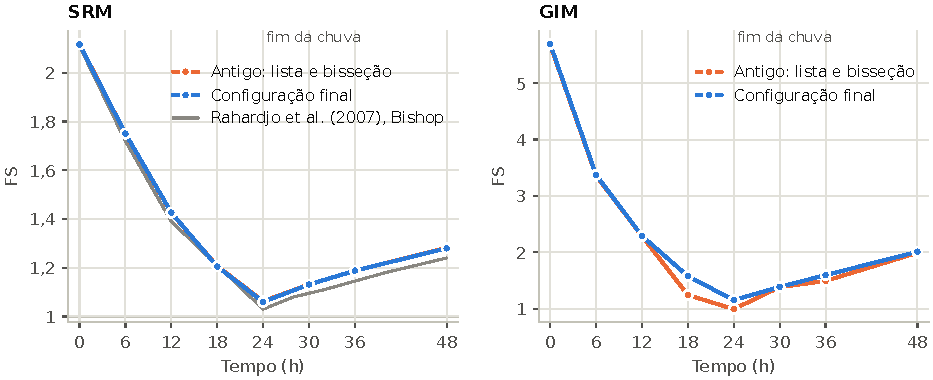
\includegraphics[width=\linewidth]{figuras/fs_tempo.pdf}
\caption{FS ao longo do tempo no caso base, pelo método antigo e pela configuração final. A curva cinza é a de Rahardjo et al.~\cite{rahardjo2007} (Bishop simplificado), digitalizada da Fig.~4 do artigo, com incerteza de cerca de $\pm 0{,}03$. As escalas de FS são diferentes nos dois painéis.}\label{fig:fs_tempo}
\end{figure}

\begin{figure}[htbp]
\centering
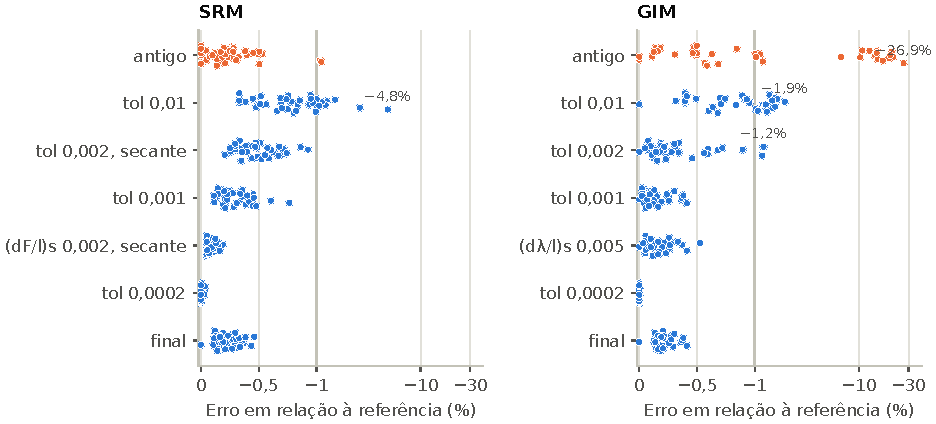
\includegraphics[width=\linewidth]{figuras/erros.pdf}
\caption{Erro em relação à referência, um ponto por caso. A escala é linear até $-1\%$, o limite de robustez, e logarítmica além disso. Só o maior erro de cada linha é rotulado, quando passa de 1\%.}\label{fig:erros}
\end{figure}

\begin{figure}[htbp]
\centering
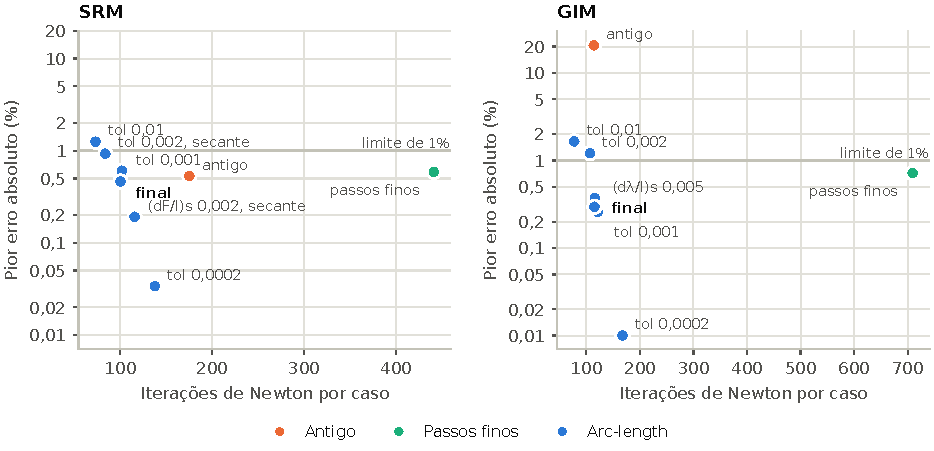
\includegraphics[width=\linewidth]{figuras/custo_erro.pdf}
\caption{Custo e pior erro nos casos que têm passos finos (16 no SRM e 15 no GIM). Melhor é para baixo e para a esquerda.}\label{fig:custo_erro}
\end{figure}

\begin{figure}[htbp]
\centering
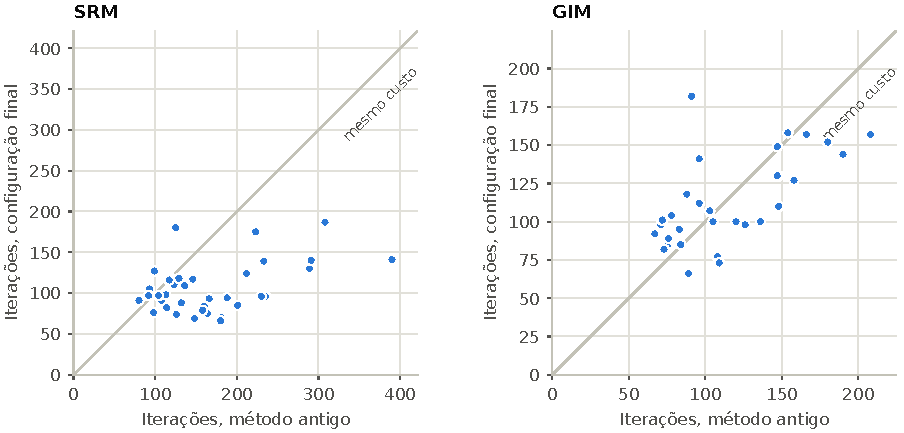
\includegraphics[width=\linewidth]{figuras/iter_antigo_novo.pdf}
\caption{Iterações de Newton por caso: método antigo contra a configuração final. Pontos abaixo da diagonal custam menos com o arc-length.}\label{fig:iter}
\end{figure}

\textbf{Tempo.} Em rodadas limpas, sem outros processos além de 4 rodadas simultâneas com um thread cada, os 8 instantes do caso base custaram: SRM antigo 325~s (1485 iterações) e SRM final 219~s (833 iterações); GIM antigo 154~s (954 iterações) e GIM final 140~s (889 iterações). O tempo por iteração foi de $0{,}22$~s no SRM antigo, $0{,}26$~s no SRM final, $0{,}16$~s no GIM antigo e $0{,}16$~s no GIM final. Assim, nesses instantes, o SRM final foi 33\% mais rápido, com 44\% menos iterações, porque cada iteração do arc-length no SRM custa mais (duas retrossubstituições e um resíduo a mais). O GIM final foi 9\% mais rápido. Com esses tempos por iteração, a economia estimada nos 38 casos é de cerca de 22\% no SRM, e não 35\%, e de cerca de 9\% no GIM.

\subsection{Triagem: quais parâmetros importam}\label{sec:triagem}

As Figuras~\ref{fig:oat_srm} e~\ref{fig:oat_gim} resumem a triagem, com um parâmetro variado de cada vez nos 5 casos. Os valores completos estão nas Tabelas~\ref{tab:oat_srm} e~\ref{tab:oat_gim}.

\begin{figure}[htbp]
\centering
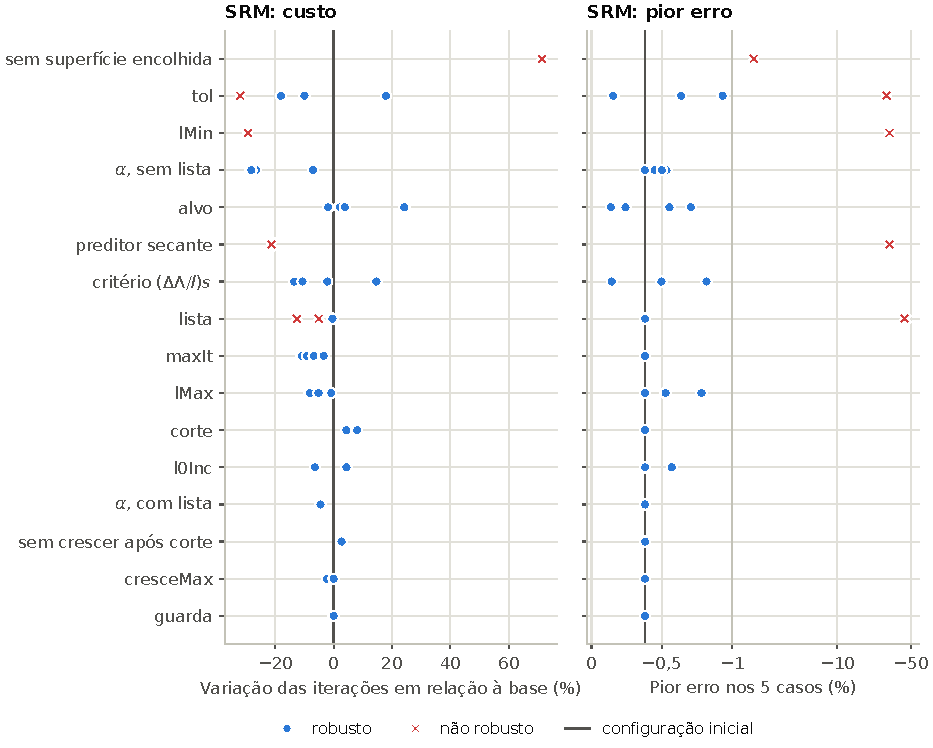
\includegraphics[width=\linewidth]{figuras/oat_srm.pdf}
\caption{Triagem do SRM. Cada ponto é um nível do parâmetro, comparado com a configuração inicial (lista, tangente, tol = 0,001, 731 iterações). As linhas estão ordenadas pelo maior efeito no custo.}\label{fig:oat_srm}
\end{figure}

\begin{figure}[htbp]
\centering
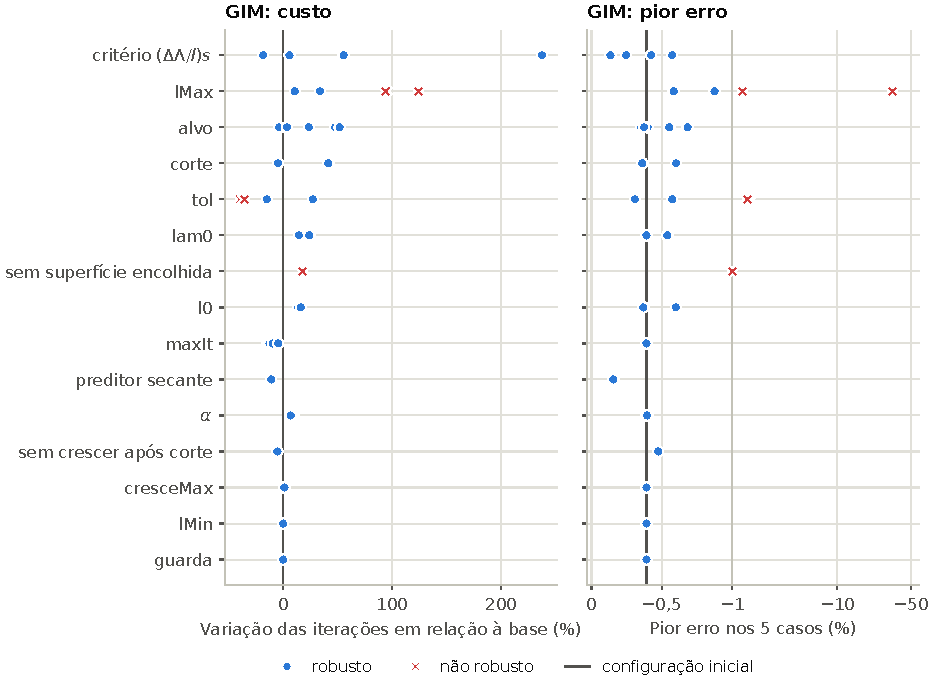
\includegraphics[width=\linewidth]{figuras/oat_gim.pdf}
\caption{Triagem do GIM, com a configuração inicial tangente e tol = 0,001 (704 iterações).}\label{fig:oat_gim}
\end{figure}

\begin{itemize}
\item \textbf{Superfície encolhida, com preditor tangente: essencial.} Sem ela, o SRM gasta 71\% mais iterações (1253 contra 731), e o pior erro vai a $-1{,}61\%$; o GIM gasta 18\% mais e chega a $-1{,}01\%$. Esse efeito vale para o preditor tangente: com secante, ela só atua no primeiro incremento, e o efeito não foi medido à parte.
\item \textbf{Lista no SRM: é a principal fonte de falhas.} Com listas que começam em $F = 1$, o caso base em 24~h falha no primeiro salto e termina em $F = F_0 = 0{,}6$ ($-43{,}53\%$). Sem lista e com $\alpha = 0{,}1$, o custo cai 29\% (522 iterações), com o mesmo erro. O resultado quase não muda entre $\alpha = 0{,}05$ e $0{,}2$.
\item \textbf{tol: controla o balanço entre custo e precisão.} A Seção~\ref{sec:parada_res} trata disso.
\item \textbf{\texttt{maxIt}: economia sem efeito no FS.} De 25 para 10, o SRM gasta 11\% menos e o GIM 15\% menos, com praticamente os mesmos valores de FS: as falhas só ficam mais baratas. Entre 10 e 12, a diferença é de 1 a 2\%, dentro do ruído, e 12 foi mantido como folga.
\item \textbf{\texttt{alvo}:} valores baixos cortam menos e fazem mais incrementos; valores altos cortam mais. No SRM, o efeito no custo fica entre $-2\%$ e $+24\%$. No GIM, \texttt{alvo} acima de 10 custa até 52\% mais. No SRM, na configuração da triagem (lista e tangente), \texttt{alvo} = 15 custou 2\% menos e errou menos ($-0{,}15\%$ contra $-0{,}38\%$); esse valor não foi testado com $\alpha$ e secante, e \texttt{alvo} = 12 não trouxe ganho nas combinações. Fica \texttt{alvo} = 10, mas esse ponto ainda pode render alguma melhora.
\item \textbf{\texttt{lMax}: valores baixos pioram o erro.} No GIM, limitar muito $l$ também encarece (+34\% com 0,1 e +124\% com 0,02), pois o patamar é longo; com 0,02, o caminho não chega ao fim em 100 incrementos, e o erro vai a $-33{,}39\%$. No SRM, todos os níveis reduzem o custo, de 1\% a 8\%, mas o pior erro vai de $-0{,}38\%$ a $-0{,}78\%$, pois $\Delta F$ fica pequeno antes de o caminho estar plano (Seção~\ref{sec:lmax}).
\item \textbf{\texttt{lMin}: muito alto é perigoso.} Com 0,01 no SRM, o caminho a partir de $F = 1$ termina logo no caso de $c' = 20$~kPa, com erro de $-31{,}36\%$.
\item \textbf{Efeito pequeno:} \texttt{cresceMax}, \texttt{corte} = 0,25, a regra de não crescer após um corte, e o termo em $\alpha$ no GIM (nesse último, 7 a 10\% mais caro e sem ganho). Por isso, ficam com o valor mais simples.
\end{itemize}

\subsection{Parada falsa e critérios de parada}\label{sec:parada_res}

O critério $\Delta\Lambda < \mathrm{tol}$ tem duas fragilidades, ambas ligadas ao fato de $\Delta\Lambda$ depender de $l$. A Figura~\ref{fig:caminho} mostra o caso normal. Como o patamar sobe devagar, a parada com tol = 0,01 fica abaixo da referência: no GIM, 0,011 abaixo de 1,154; no SRM, 0,008 abaixo de 1,063. Nesses casos, a distância é da ordem de tol, mas ela não é limitada por tol: no SRM com $c' = 0{,}5$~kPa em 48~h, chega a 0,043.

\begin{figure}[htbp]
\centering
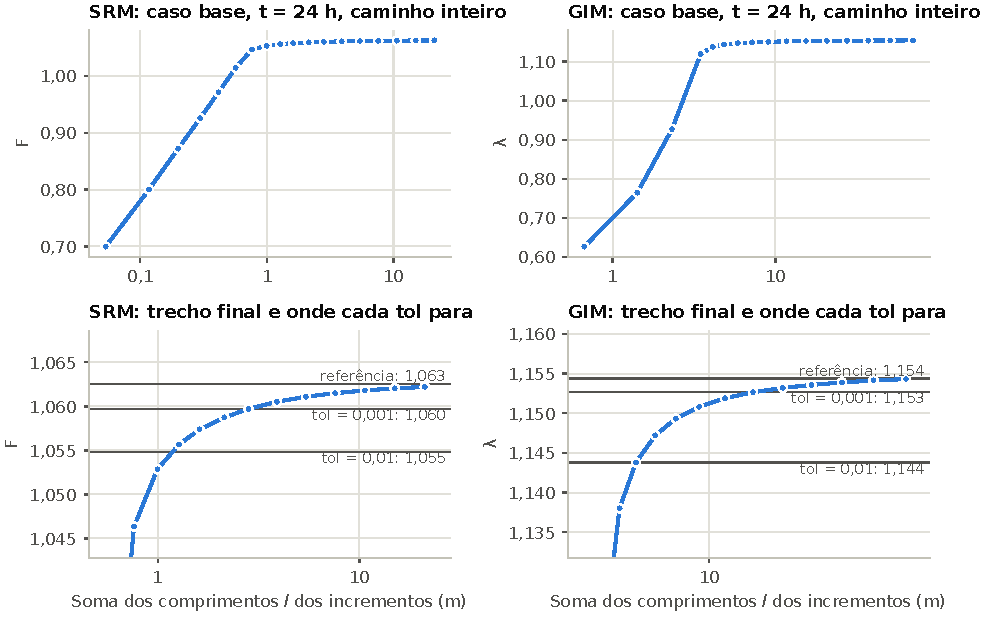
\includegraphics[width=\linewidth]{figuras/caminho.pdf}
\caption{Caminho de equilíbrio do caso base em $t = 24$~h, com a parada apertada (tol = 0,0002), e os fatores em que cada tolerância para. Cada ponto é um incremento aceito. O eixo horizontal é logarítmico.}\label{fig:caminho}
\end{figure}

\textbf{Primeira fragilidade: incremento curto logo depois da lista.} Com lista e tol = 0,01, no caso de $c' = 20$~kPa em 24~h, $F = 1$ converge e $F = 1{,}2$ falha. O arco começa com $l$ muito pequeno, herdado do passo prescrito, e dá $\Delta F$ abaixo de 0,01 em $F = 1{,}029$, enquanto o limite é 1,457 (erro de $-29{,}35\%$). A guarda não protege, pois $\Delta F/l$ cai rápido à medida que a zona plástica cresce. Esse caso motivou a retirada da lista.

\textbf{Segunda fragilidade: corte de $l$.} Sem lista, com $\alpha = 0{,}1$ e tol = 0,01, três casos de coesão muito baixa pararam cedo: $-9{,}50\%$ ($c' = 0{,}5$, 48~h), $-7{,}35\%$ ($c' = 1$, 36~h) e $-7{,}01\%$ ($c' = 0$, 12~h). Nos três, um incremento falha, $l$ cai à metade e $\Delta F$ fica abaixo de tol só por causa do corte. Medir $\Delta F$ no $l$ pedido, com \texttt{maxIt} = 12 e preditor tangente, reduz esses erros para $-4{,}85\%$, $-2{,}61\%$ e $-1{,}51\%$. O restante vem de $l$ limitado pelas falhas da Newton nesses casos, o que não se resolve com projeção. Com tol = 0,001 e secante, os três ficam abaixo de $0{,}4\%$ na configuração final.

\textbf{Alternativas testadas.}
\begin{itemize}
\item \emph{$(\Delta\Lambda/l)\,s < \mathrm{tol}$.} Não depende de $l$ e é o mais preciso no SRM: com tol = 0,002 e secante, $-0{,}19\%$ em 4581 iterações, contra $-0{,}46\%$ em 3963 da configuração final. Fica como alternativa para quem precisa de mais precisão. No GIM, não houve vantagem ($-0{,}53\%$ em 4161 iterações, contra $-0{,}41\%$ em 4141).
\item \emph{Confirmação com $\Lambda + \delta$.} Não foi adotada. Em 7 casos, com tol = 0,002 e $\delta = 0{,}002$, gastou 1032 iterações, com pior erro de $-0{,}39\%$ e erro médio de $0{,}14\%$. O critério $(\Delta\Lambda/l)\,s$ com tol = 0,002 e secante custou menos e errou menos (943 iterações, $-0{,}14\%$ e $0{,}10\%$). Além disso, a Newton pode falhar havendo equilíbrio acima: com $c' = 1$ em 36~h, tol = 0,01 e $\delta = 0{,}01$, $F = 0{,}7793$ falhou em 25 iterações a partir de $F = 0{,}7693$, e a referência é 0,790.
\item \emph{Guarda.} No SRM, nos 38 casos, tirar a guarda não mudou nenhum FS (a configuração com guarda e a final deram valores idênticos). No GIM, o mesmo ocorreu nos 5 casos em que isso foi comparado. Por isso, ela saiu do código.
\end{itemize}

\textbf{A tolerância.} O pedido inicial do estudo era tol = 0,01 no GIM. Com esse valor, o GIM economiza 34\% em relação ao antigo, mas erra mais de 1\% em 16 casos, com pior erro de $-1{,}95\%$, sempre abaixo da referência. Com tol = 0,002, ainda há 2 casos acima de 1\%. O valor tol = 0,001 com secante é o maior que atende aos critérios nos dois métodos. Com tangente, ele não basta: o pior erro é de $-0{,}77\%$ no SRM (38 casos) e de $-1{,}01\%$ no GIM (6 casos).

\subsection{Combinações de parâmetros}\label{sec:combinacoes}

A Figura~\ref{fig:fatorial} mostra todas as combinações, e as Tabelas~\ref{tab:fatorial_srm} e~\ref{tab:fatorial_gim} trazem os valores. O preditor secante age de forma diferente nos dois métodos. No GIM, com tol = 0,001, reduz custo, cortes e erro: $-0{,}41\%$ em 658 iterações e 12 cortes, contra $-1{,}01\%$ em 766 iterações e 18 cortes com tangente. No SRM, tem mais cortes (79 contra 50 nos 38 casos), e os 5\% de economia ficam dentro do ruído; o ganho é no erro, de $-0{,}77\%$ para $-0{,}46\%$. Sobre os outros parâmetros, \texttt{alvo} = 8 ou 12 não trouxe ganho, e \texttt{maxIt} = 10 custa de 1\% a 2\% menos que 12, com o mesmo pior erro.

\begin{figure}[htbp]
\centering
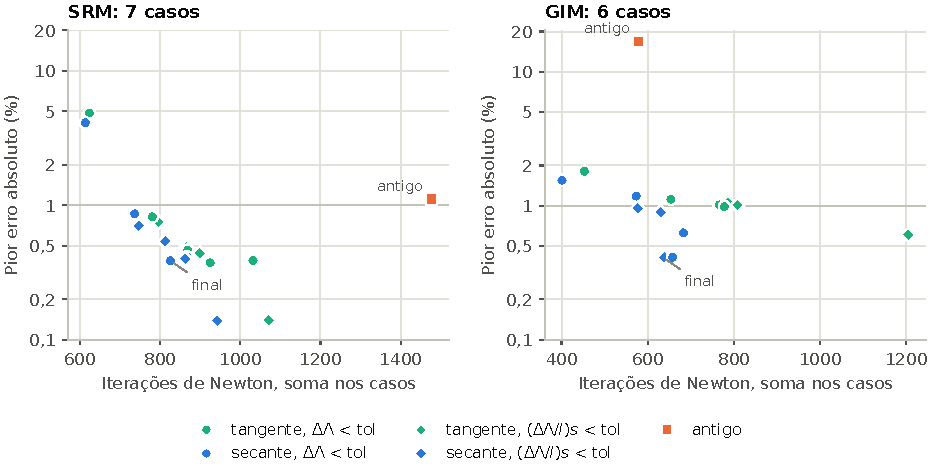
\includegraphics[width=\linewidth]{figuras/fatorial.pdf}
\caption{Combinações de critério de parada, tolerância, preditor, \texttt{alvo} e \texttt{maxIt}. O método antigo é mostrado nos mesmos casos. Com a lista fora, o SRM não tem parada falsa, mas ainda há erros grandes em tol = 0,01.}\label{fig:fatorial}
\end{figure}

Com $F_0$, há uma escolha de custo. Partir de $F_0 = 0{,}4$ em todos os casos custa 12\% mais (4420 contra 3963 iterações) e só importa quando o FS está abaixo de 0,6. Por isso, a configuração final parte de $F_0 = 0{,}6$ e só reinicia com 0,4 se o estado geostático falhar. Isso resolveu um caso em que nenhum outro método do SRM deu resposta: $c' = 0$ em 36~h, com FS = 0,555.

\subsection{Limites de $l$}\label{sec:lmax}

A Figura~\ref{fig:comprimentos} mostra os comprimentos usados. O limite inferior não é atingido: na configuração final, o menor $l/u_{\mathrm{ref}}$ aceito foi 0,0022 no SRM e 0,049 no GIM, e o menor que falhou foi 0,0045 e 0,098, muito acima de \texttt{lMin} $= 10^{-4}$. Esse valor deixa espaço para cortes em caminhos mais difíceis sem encerrar o cálculo antes da hora, e a saída por \texttt{lMin} é informada.

O limite superior tem papéis diferentes nos dois métodos. No SRM final, \texttt{lMax} = 0,5 nunca atua (o maior $l/u_{\mathrm{ref}}$ foi 0,46), e os FS são idênticos aos sem limite nos 38 casos: é só uma trava de segurança. Valores menores começam a atuar: com $F_0 = 0{,}4$, \texttt{lMax} = 0,3 muda os erros em até $0{,}065\%$. No GIM, \texttt{lMax} = 2 atua de fato: $l$ chega a esse valor em 25 de 37 das rodadas. Ele reduz os cortes de 75 para 56 e o custo em 5\%, com o mesmo pior erro, mas o erro médio sobe de $0{,}13\%$ para $0{,}21\%$. É uma escolha de custo.

\begin{figure}[htbp]
\centering
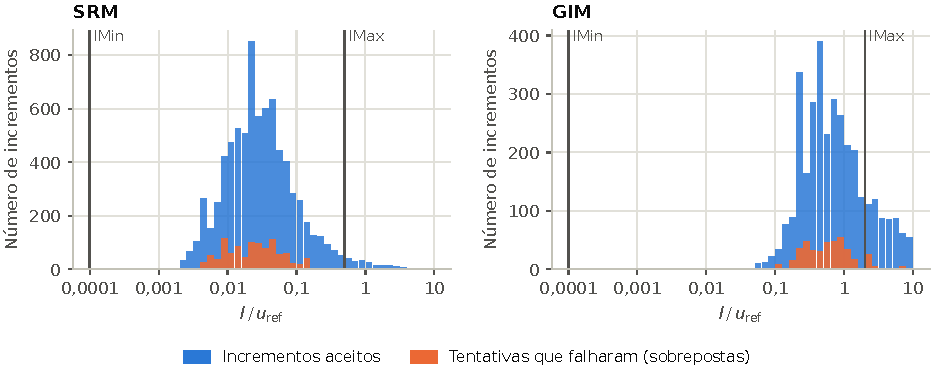
\includegraphics[width=\linewidth]{figuras/comprimentos.pdf}
\caption{Distribuição de $l/u_{\mathrm{ref}}$ nas configurações sem \texttt{lMax} dos estudos (SRM sem lista e GIM com secante), com os limites recomendados. O eixo horizontal é logarítmico.}\label{fig:comprimentos}
\end{figure}

\subsection{Reprodutibilidade e sensibilidade a pequenas mudanças}\label{sec:reprodutibilidade}

\begin{table}[htbp]
\centering\small
\caption{Perturbação dos parâmetros e reprodutibilidade da configuração final, nos 5 casos da triagem e nos dois piores casos de cada método.}\label{tab:robustez}
\begin{tabular}{llrrrrrc}
\toprule
 & Mudança & Casos & Iter. & Iter. base & Maior dif. no FS (\%) & Pior erro (\%) &  \\
\midrule
SRM & $l_0$ + 3\% & $7$ & $727$ & $705$ & $0{,}059$ & $-0{,}48$ & $\neq$ \\
SRM & $\alpha$ e $l_0$ + 3\% & $7$ & $729$ & $705$ & $-0{,}141$ & $-0{,}60$ & $\neq$ \\
SRM & 2 threads, repetição 1 & $7$ & $705$ & $705$ & $-0{,}000$ & $-0{,}46$ & $\neq$ \\
SRM & 2 threads, repetição 2 & $5$ & $512$ & $512$ & $0{,}000$ & $-0{,}28$ & $=$ \\
GIM & $l_0$ + 3\% & $7$ & $756$ & $717$ & $-0{,}115$ & $-0{,}50$ & $\neq$ \\
GIM & \texttt{lam0} + 3\% & $7$ & $754$ & $717$ & $-0{,}099$ & $-0{,}51$ & $\neq$ \\
GIM & 2 threads, repetição 1 & $7$ & $717$ & $717$ & $0{,}000$ & $-0{,}41$ & $=$ \\
GIM & 2 threads, repetição 2 & $5$ & $534$ & $534$ & $0{,}000$ & $-0{,}17$ & $=$ \\
\bottomrule
\end{tabular}
\end{table}


\textbf{Reprodutibilidade.} Com 2 threads e repetição (Tabela~\ref{tab:robustez}), o FS e o número de iterações da configuração final são idênticos aos da rodada com 1 thread, nos dois métodos, em 7 casos. A explicação é que, com o preditor secante, a tangente não é montada no estado aceito, exceto no primeiro incremento, em que a superfície encolhida resolve o empate. O GIM antigo não tem essa propriedade. Com 1 thread, ele repetiu os mesmos valores nos 8 instantes do caso base. Com 2 threads, no caso base em 12~h, deu 1,992 em uma execução e 2,289 em duas; em 30~h, deu 0,992 nas três, contra 1,383 com 1 thread. As estatísticas das Tabelas~\ref{tab:validacao_srm} e~\ref{tab:validacao_gim} foram medidas com 1 thread, e por isso um GIM antigo com mais threads pode ficar ainda pior ou um pouco melhor. Ele também muda com o arredondamento das pressões de entrada (Seção~\ref{sec:acoplado_conf}).

\textbf{Pequenas mudanças de parâmetros.} Uma perturbação de 3\% em $l_0$, $\alpha$ ou \texttt{lam0} muda o FS em no máximo $0{,}14\%$, nos 5 casos da triagem e nos dois piores casos de cada método. Isso basta para atravessar o limite de precisão: o pior erro vai a $-0{,}60\%$ no SRM e a $-0{,}51\%$ no GIM. Portanto, a robustez (1\%) é firme, mas o rótulo ``preciso'' ($0{,}5\%$) não é: o erro esperado está perto de $0{,}5\%$ nos piores casos, e não sempre abaixo disso.

O custo por caso é menos estável, pois um pequeno desvio muda onde caem as falhas: em um caso do GIM, 84 iterações viraram 132. Em soma nos 5 casos da triagem, a variação é de até 8\%. Diferenças de custo entre configurações abaixo de cerca de 10\% não devem ser levadas a sério.

\subsection{Malha fina}\label{sec:fina}

Na malha fina (34\,658 equações), a configuração final se comporta como na malha base. No SRM, o erro é de $-0{,}30\%$ em $t = 0$ e de $-0{,}32\%$ em 24~h. No GIM, é de $-0{,}14\%$ e $-0{,}36\%$, enquanto o método antigo fica em 0,992 contra 1,102 em 24~h. Os parâmetros são adimensionais, e nada precisou ser ajustado. O custo oscila caso a caso: 199 iterações contra 111 do método antigo no SRM em $t = 0$, e 101 contra 129 em 24~h.

\subsection{Limitações}\label{sec:limitacoes}

\begin{itemize}
\item \textbf{O GIM nem sempre tem limite.} Com $\beta = 26{,}6^\circ$ em $t = 0$, a inclinação é próxima de $\phi'$. A explicação provável é que o solo ganha resistência por atrito junto com o peso. Sem teto, o caminho sobe até $\lambda \approx 4444$, sem ruptura no sentido usual. O método antigo para em 10, o fim da lista. Por isso, o código final encerra em \texttt{fatorMax} = 10 e informa. As estatísticas tratam esse caso como ``FS $\ge 10$''.
\item \textbf{O GIM pode não achar o primeiro equilíbrio.} Com $c' \le 1$~kPa, nos 6 casos testados, durante e depois da chuva (nenhum em $t = 0$), a Newton não converge no primeiro passo para nenhum $\lambda$ de 0,5 a 0,0156. Todas as variantes do GIM, nova e antiga, retornam FS = 0, enquanto o SRM dá valores entre 0,55 e 0,93 em 5 deles. Uma explicação provável é que a sucção mantida não se equilibra com o peso reduzido, mas a falha da Newton não prova que não existe equilíbrio. Nessas condições, o GIM não forneceu um FS útil.
\item \textbf{Há um caso sem resposta no SRM.} Com $c' = 0$ em 24~h, o estado geostático falha mesmo com $F_0 = 0{,}4$, e a função retorna $-1$. A causa não foi isolada: também há $p_w > 0$ perto da superfície em 12, 36 e 48~h, instantes em que o estado geostático converge, e em 36~h isso depende de $F_0$, enquanto o ápice de tração não depende de $F$.
\item \textbf{A referência é uma cota inferior.} Ela é o maior fator encontrado, e o limite verdadeiro pode estar um pouco acima. Pelo arc-length apertado, a cauda ainda sobe devagar.
\item \textbf{O erro não é limitado por tol, e a folga é pequena.} Com tol = 0,001, o pior erro foi de $0{,}46\%$ no SRM, mas a variante com $F_0 = 0{,}4$ chega a $-0{,}50\%$, e uma perturbação de 3\% passa desse valor. Extrapolando a cauda da rodada apertada com o estimador $(\Delta\Lambda/l)\,s$, os dois piores casos do SRM ficam em $-0{,}52\%$. Além disso, os mesmos casos serviram para escolher e validar, então estes números tendem a ser otimistas.
\item \textbf{Tempo.} Só foi medido em rodadas limpas no caso base. O valor para os 38 casos é uma estimativa.
\item \textbf{Escopo.} Todos os casos usam o mesmo tipo de geometria e o modelo com esqueleto rígido e ar passivo. O modelo acoplado foi testado à parte, só no caso base (Seção~\ref{sec:acoplado}).
\item \textbf{Custo do estado geostático.} As iterações do estado geostático, comuns a todos os métodos do SRM, não entram na contagem. Elas são poucas (4 incrementos).
\end{itemize}

\subsection{Parâmetros recomendados}\label{sec:recomendacao}

A Tabela~\ref{tab:recomendados} traz os valores adotados, que são os padrões das funções \texttt{ParamsSRM} e \texttt{ParamsGIM} no código do estudo (Apêndice~\ref{ap:reproducao}). Eles foram validados com o programa final em todos os 43 casos, e os valores de FS coincidem com os do estudo em todos os casos comparáveis.

\begin{table}[htbp]
\centering\small
\caption{Parâmetros recomendados.}\label{tab:recomendados}
\begin{tabular}{lccp{7.2cm}}
\toprule
Parâmetro & SRM & GIM & Razão \\
\midrule
Parada & \multicolumn{2}{c}{$\Delta\Lambda$ no $l$ pedido $< \mathrm{tol}$} & critério direto; um corte de $l$ não conta \\
\texttt{tol} & 0,001 & 0,001 & maior valor que atende aos critérios, com secante \\
Preditor & \multicolumn{2}{c}{secante} & menos erro nos dois; no GIM, também menos custo e cortes \\
Superfície encolhida & \multicolumn{2}{c}{sim, $10^{-6}$} & com secante, só no 1.\textsuperscript{o} incremento; indispensável com tangente \\
\texttt{alpha} & 0,1 & 0 & no SRM, dispensa a lista e o caminho vertical \\
\texttt{lista} & vazia & -- & principal fonte de falhas \\
\texttt{l0} & 0,01 & 0,25 & SRM: $\Delta F \approx 0{,}1$ no início \\
\texttt{F0} / \texttt{F0Min} & 0,6 / 0,4 & -- & 0,4 só se o estado geostático falhar \\
\texttt{lam0} & -- & 0,5 & menor custo entre 0,25, 0,5 e 1 \\
\texttt{alvo} & 10 & 10 & 8 e 12 não trazem ganho; 15 não testado com secante \\
\texttt{maxIt} & 12 & 12 & falhas mais baratas; 10 custa 1--2\% menos, 12 dá folga \\
\texttt{lMax} & 0,5 & 2 & SRM: só trava; GIM: menos cortes e custo, erro médio maior \\
\texttt{lMin} & $10^{-4}$ & $10^{-4}$ & nunca atingido; 0,01 causou parada falsa com lista \\
\texttt{cresceMax}, \texttt{reduzMax} & 2; 0,5 & 2; 0,5 & \texttt{cresceMax}: efeito pequeno; \texttt{reduzMax}: não variado \\
\texttt{corte} & 0,5 & 0,5 & efeito pequeno no SRM; 0,75 custa 41\% mais no GIM \\
\texttt{fatorMax} & 10 & 10 & evita percorrer caminhos sem limite \\
\texttt{maxPassos} & 100 & 100 & limite de segurança; nunca atingido \\
\bottomrule
\end{tabular}
\end{table}


\section{Teste no modelo acoplado com ar ativo}\label{sec:acoplado}

Os parâmetros da Seção~\ref{sec:recomendacao} foram escolhidos com esqueleto rígido e ar passivo. Esta seção aplica os mesmos valores, sem nenhum ajuste, ao modelo completo, chamado aqui de \emph{modelo i}. Os campos de pressão deste teste não participaram da escolha dos parâmetros, mas o solo, a malha e a geometria são os do caso base. Portanto, ele testa outro modelo físico, não outras geometrias.

\subsection{O modelo i}\label{sec:modelo_i}

O modelo i resolve $\mathbf{u}$, $p_w$ e $p_a$ juntos em cada passo de tempo, com o mesmo $\Delta t$. Além do equilíbrio~\eqref{eq:equilibrio}, valem os balanços de massa da água e do ar, com grãos incompressíveis:
\begin{align}
S_w\,\dot\varepsilon_v + n\,\dot S_w + \frac{n S_w}{K_w}\,\dot p_w + \nabla\cdot\mathbf{q}_w &= 0,\\
S_a\,\dot\varepsilon_v + n\,\dot S_a + \frac{n S_a}{p_{\mathrm{abs}}}\,\dot p_a + \nabla\cdot\mathbf{q}_a + \frac{\mathbf{q}_a\cdot\nabla p_a}{p_{\mathrm{abs}}} &= 0,
\end{align}
com $S_a = 1 - S_w$, $p_{\mathrm{abs}} = p_a + p_{\mathrm{atm}}$ e
\begin{equation}
\mathbf{q}_w = -\frac{k_s\,k_{rw}}{\gamma_w}\big(\nabla p_w - \gamma_w\mathbf{g}\big), \qquad
\mathbf{q}_a = -\frac{\mu_w}{\mu_a}\,\frac{k_s\,k_{ra}}{\gamma_w}\big(\nabla p_a - \gamma_a\mathbf{g}\big).
\end{equation}
Os valores do ar são hipóteses do código, pois o artigo não modela o ar: $k_{ra} = (1 - S_w)^2\,(1 - S_w^{5/3})$, com piso de $10^{-4}$, $\mu_w/\mu_a = 10^{-3}/(1{,}8\times10^{-5})$, $\gamma_a = 1{,}2\times 9{,}81\times 10^{-3}$~kN/m$^3$ e $p_{\mathrm{atm}} = 101{,}325$~kPa. Em relação ao modelo rígido, muda o seguinte:
\begin{itemize}
\item \textbf{Mecânica:} $\mathbf{u}$ é livre, com os mesmos apoios, e o equilíbrio entra em cada passo, com $c'/F_{\mathrm{tr}}$, $\tan\phi'/F_{\mathrm{tr}}$ e $\tan\psi/F_{\mathrm{tr}}$. O fator $F_{\mathrm{tr}}$ é a variável \texttt{F\_TRANS} do código.
\item \textbf{Ar:} $p_a$ é livre, com $p_a = 0$ só na superfície. A base e as laterais são fechadas ao ar.
\item \textbf{Água:} as condições de contorno são as mesmas, inclusive a face de percolação.
\item \textbf{Estado inicial:} o mesmo $p_w$ hidrostático, com $p_a = 0$. O peso entra em 4 incrementos, com a resistência real, e os deslocamentos são zerados, mantendo as tensões.
\item \textbf{Passo que falha:} é dividido ao meio, até 4 vezes.
\end{itemize}

Foram usados dois valores de $F_{\mathrm{tr}}$. Com $F_{\mathrm{tr}} = 1$, o transiente usa a resistência real, e o talude plastifica quando chega ao limite. Com $F_{\mathrm{tr}} = 0{,}5$, $c'$ e $\tan\phi'$ dobram no transiente: pelas medidas do projeto \texttt{SlopeRandomField}, nenhum ponto plastifica, e o acoplamento elástico e o ar continuam. É um artifício para deixar o FS livre para cair abaixo de 1, não um solo real. O maior deslocamento do transiente foi de 19~cm com $F_{\mathrm{tr}} = 1$ e de 6~cm com $F_{\mathrm{tr}} = 0{,}5$.

O FS é calculado como na Seção~\ref{sec:fs_congelado}, para qualquer $F_{\mathrm{tr}}$: $p_w$ e $p_a$ ficam congelados, e o cálculo parte do estado sem tensões, com a resistência real. Assim, a história plástica do transiente não entra no FS, só as pressões. Como $\chi = 1$, tem-se $p_B = p_w$, e $p_a$ não aparece no equilíbrio: o ar afeta o FS só por meio de $p_w$.

Duas propriedades servem de conferência. Primeira: com $F = 1$ e $\lambda = 1$, o problema é o mesmo nos dois métodos, então o SRM e o GIM devem ficar do mesmo lado de 1. Segunda: com $F_{\mathrm{tr}} = 1$, cada estado do transiente já está em equilíbrio com a resistência real, para aquelas pressões. Com fluxo associado, o teorema do limite inferior dá FS $\ge 1$ nos dois métodos. Com $F_{\mathrm{tr}} = 0{,}5$, não há essa garantia.

\subsection{Rodadas}

Há um transiente para cada $F_{\mathrm{tr}}$, com o solo f50 e chuva de 36~mm/h por 24~h. O FS é calculado a cada 6~h, de 0 a 48~h. São 18 cálculos por método, em 17 instantes distintos, pois $t = 0$ é igual nos dois transientes. Os métodos são:
\begin{itemize}
\item a configuração final;
\item o arc-length apertado (tol = 0,0002, \texttt{maxIt} = 25 e sem \texttt{lMax}, como no estudo);
\item o método antigo, de lista e bisseção, com as mesmas funções do estudo;
\item só no SRM, a lista densa usada no Monte Carlo ($F$ de 0,1 em 0,1 a partir de 0,7, com nova tentativa), de rodadas anteriores com as mesmas pressões.
\end{itemize}
A referência é o maior FS do instante entre os métodos da família, como na Seção~\ref{sec:estudo}. Todas as rodadas usam 1 thread.

\subsection{Resultados}\label{sec:acoplado_res}

\begin{table}[htbp]
\centering\small
\caption{FS ao longo do tempo com a configuração final, no solo f50 com 36~mm/h por 24~h. O modelo rígido não tem rodada em 42~h. A última coluna é o maior $p_a$ no domínio, com $F_{\mathrm{tr}} = 0{,}5$.}\label{tab:acoplado_fs}
\begin{tabular}{r*{6}{>{\raggedleft\arraybackslash}p{1.2cm}}r}
\toprule
 & \multicolumn{2}{c}{Rígido, ar passivo} & \multicolumn{2}{c}{Modelo i, $F_{\mathrm{tr}} = 1$} & \multicolumn{2}{c}{Modelo i, $F_{\mathrm{tr}} = 0{,}5$} & $p_{a,\max}$ \\ \cmidrule(lr){2-3}\cmidrule(lr){4-5}\cmidrule(lr){6-7} $t$ (h) & SRM & GIM & SRM & GIM & SRM & GIM & (kPa) \\
\midrule
$0$ & $2{,}116$ & $5{,}696$ & $2{,}116$ & $5{,}696$ & $2{,}116$ & $5{,}696$ & $0{,}0$ \\
$6$ & $1{,}751$ & $3{,}374$ & $1{,}476$ & $2{,}428$ & $1{,}470$ & $2{,}400$ & $30{,}5$ \\
$12$ & $1{,}426$ & $2{,}290$ & $1{,}110$ & $1{,}311$ & $1{,}096$ & $1{,}265$ & $43{,}6$ \\
$18$ & $1{,}205$ & $1{,}577$ & $1{,}020$ & $1{,}056$ & $1{,}001$ & $1{,}008$ & $47{,}7$ \\
$24$ & $1{,}060$ & $1{,}153$ & $1{,}005$ & $1{,}018$ & $0{,}963$ & $0{,}920$ & $52{,}9$ \\
$30$ & $1{,}131$ & $1{,}386$ & $1{,}171$ & $1{,}572$ & $1{,}158$ & $1{,}518$ & $50{,}3$ \\
$36$ & $1{,}188$ & $1{,}596$ & $1{,}316$ & $2{,}240$ & $1{,}307$ & $2{,}200$ & $42{,}1$ \\
$42$ & -- & -- & $1{,}432$ & $2{,}767$ & $1{,}426$ & $2{,}742$ & $35{,}8$ \\
$48$ & $1{,}280$ & $2{,}010$ & $1{,}515$ & $3{,}130$ & $1{,}512$ & $3{,}111$ & $31{,}4$ \\
\bottomrule
\end{tabular}
\end{table}


\begin{figure}[htbp]
\centering
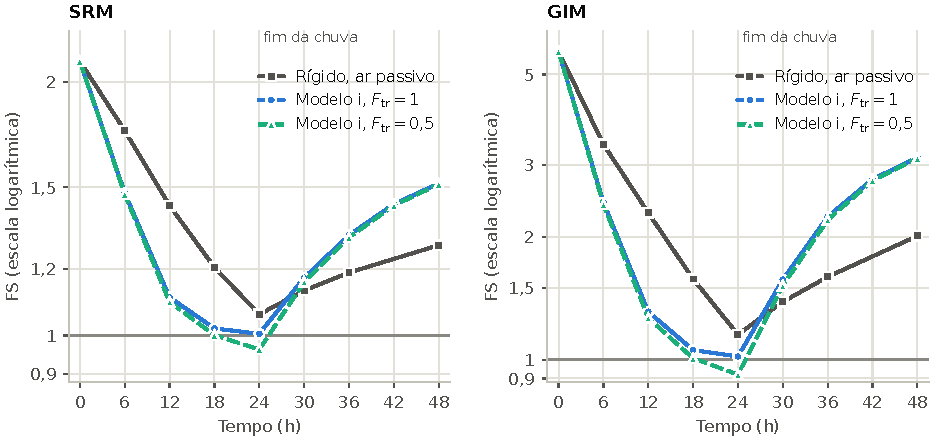
\includegraphics[width=\linewidth]{figuras/acoplado_fs.pdf}
\caption{FS ao longo do tempo com a configuração final, no modelo rígido e no modelo i. O eixo de FS é logarítmico, com escalas diferentes nos dois painéis, e a linha horizontal marca FS = 1. O modelo rígido não tem rodada em 42~h.}\label{fig:acoplado_fs}
\end{figure}

A Tabela~\ref{tab:acoplado_fs} e a Figura~\ref{fig:acoplado_fs} mostram o FS ao longo do tempo.

\textbf{Efeito do ar.} Durante a chuva, o FS cai bem mais cedo que no modelo rígido: em 12~h, o SRM dá $1{,}110$ com $F_{\mathrm{tr}} = 1$ e $1{,}096$ com $F_{\mathrm{tr}} = 0{,}5$, contra $1{,}426$ no rígido. De 30~h em diante, fica acima do rígido. O menor FS continua em 24~h, e o maior $p_a$ no domínio chega a $52{,}9$~kPa. A diferença vem principalmente do ar, não da deformação: com o SRM de lista densa, a variante acoplada com $p_a = 0$ dá 1,081 em 24~h, perto dos 1,0625 do modelo rígido, enquanto o modelo i com $F_{\mathrm{tr}} = 0{,}5$ dá 0,9625 (\texttt{README.md} de \texttt{SlopeRandomField}). Esse efeito depende do modelo do ar: com piso de $k_{ra}$ igual a 0,01, a mesma busca deu 1,006 em 24~h, acima de 1. Esse caso não foi repetido com arc-length. Por isso, FS abaixo de 1 no modelo i não é uma conclusão firme sobre o talude.

\textbf{$F_{\mathrm{tr}} = 1$.} Nenhum valor fica abaixo de 1, nos dois métodos, como o limite inferior prevê. O mínimo está em 24~h: $1{,}005$ no SRM (referência de $1{,}008$) e $1{,}018$ no GIM (referência de $1{,}020$). O SRM antigo dá $1{,}000$ nesse instante, $-0{,}77\%$ em relação à referência. Assim, um FS exatamente igual a 1 era limitação da busca: o talude está perto do limite, mas o FS fica um pouco acima. O limiar FS $< 1{,}01$, usado com o SRM de lista nessas rodadas para identificar o talude no limite, não se transfere ao GIM.

\textbf{$F_{\mathrm{tr}} = 0{,}5$.} Só o instante de 24~h fica abaixo de 1: $0{,}963$ no SRM e $0{,}920$ no GIM. Em 18~h, os dois estão pouco acima: $1{,}001$ e $1{,}008$.

\textbf{Os dois métodos.} Com a configuração final, o SRM e o GIM ficam do mesmo lado de 1 nos 18 cálculos. O GIM antigo fica do lado errado em 3 deles. Com $F_{\mathrm{tr}} = 1$, dá $0{,}992$ em 18~h e $0{,}992$ em 24~h, o que contraria o limite inferior. Com $F_{\mathrm{tr}} = 0{,}5$, dá $0{,}992$ em 18~h, contra $1{,}008$ da configuração final. Longe de 1, os valores dos dois métodos não se comparam (Seção~\ref{sec:fs_congelado}).

\begin{table}[htbp]
\centering\footnotesize\setlength{\tabcolsep}{3pt}
\caption{Custo e erro no modelo i, nos 18 cálculos (9 instantes em cada transiente; $t = 0$ é igual nos dois). A referência é o maior FS do instante entre todos os métodos da família. ``It. (1)'' e ``It. (0,5)'' são as iterações com $F_{\mathrm{tr}} = 1$ e $0{,}5$, e ``It.'' é a soma. ``Rel.'' é a variação das iterações em relação ao método antigo.}\label{tab:acoplado_erro}
\begin{tabular}{p{3.7cm}rrrrrrrrcc}
\toprule
Método & It. (1) & It. (0,5) & It. & Rel. (\%) & Pior (\%) & Méd. (\%) & $>0{,}5\%$ & $>1\%$ & Rob. & Prec. \\
\midrule
SRM, antigo & $1\,413$ & $1\,191$ & $2\,604$ & -- & $-0{,}77$ & $0{,}27$ & $2$ & $0$ & sim & \textbf{não} \\
SRM, lista densa & $1\,260$ & $1\,090$ & $2\,350$ & $-10$ & $-0{,}77$ & $0{,}30$ & $3$ & $0$ & sim & \textbf{não} \\
\textbf{SRM, final} & $903$ & $892$ & $1\,795$ & $-31$ & $-0{,}41$ & $0{,}23$ & $0$ & $0$ & sim & sim \\
SRM, arc-length apertado & $1\,268$ & $1\,244$ & $2\,512$ & $-4$ & $-0{,}02$ & $0{,}00$ & $0$ & $0$ & sim & sim \\
\midrule
GIM, antigo & $987$ & $1\,071$ & $2\,058$ & -- & $-20{,}58$ & $5{,}90$ & $15$ & $14$ & \textbf{não} & \textbf{não} \\
\textbf{GIM, final} & $1\,120$ & $1\,161$ & $2\,281$ & $+$$11$ & $-0{,}29$ & $0{,}23$ & $0$ & $0$ & sim & sim \\
GIM, arc-length apertado & $1\,663$ & $1\,631$ & $3\,294$ & $+$$60$ & $0{,}00$ & $0{,}00$ & $0$ & $0$ & sim & sim \\
\bottomrule
\end{tabular}
\end{table}


\textbf{Erro.} A Tabela~\ref{tab:acoplado_erro} resume custo e erro, e os valores por instante estão no Apêndice~\ref{ap:tabelas}. Os parâmetros continuaram valendo. No SRM, o pior erro é de $-0{,}41\%$ e o médio é de $0{,}23\%$, contra $-0{,}46\%$ e $0{,}23\%$ nos 38 casos do estudo. No GIM, são $-0{,}29\%$ e $0{,}23\%$, contra $-0{,}41\%$ e $0{,}21\%$. Os 18 cálculos de cada método pararam pelo critério, com 26 cortes de $l$ no SRM e 40 no GIM. O SRM antigo chega a $-0{,}77\%$, com 2 cálculos acima de $0{,}5\%$. O GIM antigo fica mais de 1\% abaixo da referência em 14 dos 18 cálculos, com pior erro de $-20{,}58\%$.

\textbf{Custo.} O SRM final gasta 1795 iterações: 31\% menos que o antigo (2604) e 24\% menos que a lista densa (2350). O antigo gasta menos em 3 dos 18 cálculos. O GIM final gasta 2281 iterações, 11\% mais que o antigo (2058), que é mais barato porque para cedo. O arc-length apertado custa 40\% mais que a configuração final no SRM e 44\% mais no GIM.

\textbf{Tempo.} Com 2 processos simultâneos de 1 thread, cada cálculo final levou de 19 a 38~s no SRM e de 14 a 28~s no GIM. Em soma nos 18 cálculos, o SRM final levou 454~s, contra 562~s do antigo (19\% menos), e o GIM final levou 347~s, contra 337~s (3\% mais). A máquina não estava reservada, então esses tempos são só indicativos. Cada transiente levou cerca de 9~min com $F_{\mathrm{tr}} = 1$ e 6~min com $F_{\mathrm{tr}} = 0{,}5$.

\subsection{Conferências}\label{sec:acoplado_conf}

\begin{itemize}
\item \textbf{Instante inicial.} Em $t = 0$, as pressões são as do modelo rígido. O FS e as iterações da configuração final e do SRM antigo são iguais aos do estudo.
\item \textbf{GIM antigo em $t = 0$.} Aqui houve diferença: $5{,}648$ com 197 iterações, contra $5{,}680$ com 180 no estudo. O programa do estudo ainda dá o seu valor, e rodar o GIM antigo sem o SRM antes dele no mesmo processo não muda o resultado. A causa é o arredondamento: o estudo lê as pressões com 10 dígitos, e este teste, com 17. Arredondar o estado para 10 dígitos, uma mudança de no máximo $5\times10^{-8}$~kPa, leva o GIM antigo a $5{,}680$ com 180 iterações. Já o GIM final dá o mesmo FS, nos 10 dígitos gravados, e as mesmas iterações nos dois casos.
\item \textbf{Transiente.} Nos 9 instantes, $p_w$ e $p_a$ coincidem com os das rodadas anteriores de \texttt{SlopeRandomField}, em todos os dígitos gravados. Foram 480 passos, sem nenhum dividido. As iterações de Newton são iguais com $F_{\mathrm{tr}} = 0{,}5$ (2239) e quase iguais com $F_{\mathrm{tr}} = 1$ (3193 contra 3171).
\item \textbf{Estados gravados.} Recalcular o FS a partir do estado gravado em 24~h, com $F_{\mathrm{tr}} = 0{,}5$, reproduz a rodada completa em todos os dígitos gravados.
\end{itemize}

\subsection{Limites deste teste}

\begin{itemize}
\item Só o solo f50, a chuva de 36~mm/h e a malha base foram usados. Outras geometrias, outros solos e a malha fina ficaram de fora.
\item O transiente não dividiu nenhum passo, então essa parte do programa não foi exercitada.
\item A referência é o mesmo método com parada mais rigorosa e uma cota inferior do limite, com a mesma ressalva da Seção~\ref{sec:limitacoes}. O limite de $0{,}5\%$ continua sem garantia, pois a perturbação da Seção~\ref{sec:reprodutibilidade} não foi repetida aqui.
\end{itemize}


\section{Conclusões}\label{sec:conclusoes}

\begin{enumerate}
\item \textbf{Com os parâmetros certos, o arc-length é melhor nos dois métodos.} No SRM, a configuração final gasta 35\% menos iterações que o método antigo (cerca de 22\% menos de tempo, por estimativa), com pior erro de $-0{,}46\%$ contra $-1{,}11\%$. No GIM, o custo é parecido (7\% menos iterações), mas o pior erro cai de $-26{,}87\%$ para $-0{,}41\%$.
\item \textbf{O GIM antigo não é confiável.} Com 1 thread, ele fica mais de 1\% abaixo da referência em 18 de 35 casos, e, com 2 threads, o resultado varia de uma execução para outra; ele muda até com o arredondamento das pressões de entrada. O padrão dos valores indica que a Newton falha em saltos da lista, abaixo do limite: os FS ficam logo abaixo de valores da lista.
\item \textbf{O que mais pesou:} no SRM, o termo em $\alpha$ no lugar da lista, que elimina a principal fonte de falhas; nos dois métodos, o preditor secante, que evita montar a tangente ambígua no estado aceito.
\item \textbf{O critério $\Delta\Lambda < \mathrm{tol}$ serve, com tol = 0,001, medido no $l$ pedido e com secante.} Com tol = 0,01, o erro passa de 1\% em vários casos nos dois métodos e chega a cerca de 5\% no SRM com coesão muito baixa. O limite de 1\% é atendido com folga. O de $0{,}5\%$ não é garantido.
\item \textbf{\texttt{lMax} e \texttt{lMin}.} Valores restritivos prejudicam o resultado: \texttt{lMax} baixo piora o erro, e \texttt{lMin} alto causou parada falsa com lista. No SRM, \texttt{lMax} = 0,5 é só uma trava; no GIM, \texttt{lMax} = 2 é uma escolha de custo.
\item \textbf{O GIM tem limites próprios.} Em um talude pouco inclinado, seu caminho não mostrou limite prático. Com coesão muito baixa, não foi possível obter o primeiro estado de equilíbrio. O SRM deu resposta em todos os casos, menos um.
\item \textbf{Os parâmetros também valem no modelo acoplado.} Sem nenhum ajuste, no modelo i com ar ativo, todos os cálculos pararam pelo critério, com pior erro de $-0{,}41\%$ no SRM e $-0{,}29\%$ no GIM. Com $F_{\mathrm{tr}} = 1$, os dois métodos ficam acima de 1, como o limite inferior prevê; com $F_{\mathrm{tr}} = 0{,}5$, só o instante de 24~h fica abaixo de 1. O GIM antigo dá 0,992 onde o limite inferior garante FS $\ge 1$.
\end{enumerate}

Os próximos passos naturais são testar estes parâmetros nas séries paramétricas do artigo, com outras alturas e inclinações, e no modelo acoplado com outros solos e chuvas. Como os casos do estudo de sensibilidade serviram tanto para escolher quanto para validar, e o teste da Seção~\ref{sec:acoplado} muda só o modelo físico, essas séries serão o primeiro teste independente em geometria.


\begin{thebibliography}{9}
\bibitem{rahardjo2007} RAHARDJO, H.; ONG, T.~H.; REZAUR, R.~B.; LEONG, E.~C. Factors controlling instability of homogeneous soil slopes under rainfall. \emph{Journal of Geotechnical and Geoenvironmental Engineering}, v.~133, n.~12, p.~1532--1543, 2007. DOI: 10.1061/(ASCE)1090-0241(2007)133:12(1532).
\bibitem{souzaneto2008} DE SOUZA NETO, E.~A.; PERI\'C, D.; OWEN, D.~R.~J. \emph{Computational Methods for Plasticity: Theory and Applications}. Chichester: John Wiley \& Sons, 2008.
\bibitem{song1997} SONG, E. Finite element analysis of safety factor for soil structures. \emph{Chinese Journal of Geotechnical Engineering}, v.~19, n.~2, p.~1--7, 1997. Em chinês.
\bibitem{sysala2025} SYSALA, S.; B\v{E}RE\v{S}, M.; B\v{E}RE\v{S}OV\'A, S.; HASLINGER, J.; KRU\v{Z}\'IK, J.; LUBER, T. Convex optimization problems inspired by geotechnical stability analysis. \emph{SIAM Journal on Optimization}, v.~35, n.~3, p.~1993--2016, 2025. DOI: 10.1137/25M1723177.
\end{thebibliography}


\appendix

\section{Reprodução}\label{ap:reproducao}

Os arquivos do estudo estão em \texttt{\textasciitilde/projects/runs/arc\_length\_sensibilidade/}, com um \texttt{README.md}:
\begin{itemize}
\item \texttt{codigo/resultados.csv}: uma linha por rodada, com caso, método, parâmetros, FS, iterações, cortes, motivo da parada e tempos. \texttt{codigo/logs/} tem os incrementos de cada rodada.
\item \texttt{codigo/}: o programa do estudo (\texttt{sens.cpp}, \texttt{main\_novo.cpp}, \texttt{lib/}), a verificação do código final (\texttt{verif\_final.cpp}, \texttt{final/}), o plano (\texttt{plano.py}, com os arquivos \texttt{.json} de cada etapa), os casos (\texttt{casos/}, \texttt{gera\_pw.cpp}), a compilação (\texttt{compilar.sh}) e os geradores deste relatório (\texttt{gera.py}, \texttt{numeros.py}, \texttt{monta.py}, \texttt{secoes/}).
\item \texttt{arco/pw\_todos.csv}: os campos de $p_w$ do caso base.
\item \texttt{medidas\_complementares/}: as medidas citadas no texto que não estão em \texttt{resultados.csv}: o ápice de tração da face de percolação, a classificação dos pontos sobre a superfície e a dispersão do arc-length antes da superfície encolhida.
\end{itemize}
Cada etapa roda com \texttt{plano.py <etapa> -{}-config <arquivo.json> -{}-procs N}. As rodadas já feitas não são repetidas. As tabelas e figuras deste relatório são geradas por \texttt{gera.py}, de \texttt{resultados.csv} e, na Seção~\ref{sec:acoplado}, dos CSV do modelo acoplado, sem números digitados à mão. O programa do estudo usa a \texttt{libpz.so} compilada do repositório, com a sua própria cópia de \texttt{TPZUnsatAnalysis}.

O teste no modelo acoplado (Seção~\ref{sec:acoplado}) está em \texttt{\textasciitilde/projects/runs/arc\_length\_ar\_ativo/}, também com um \texttt{README.md}: o programa \texttt{ar\_ativo.cpp} e, em \texttt{ftrans1/} e \texttt{ftrans0.5/}, os FS (\texttt{fs\_arco.csv}, \texttt{fs\_apertado.csv}, \texttt{fs\_antigo.csv} e \texttt{mc\_fs.csv}), o transiente e os estados de cada instante. A conferência do arredondamento está em \texttt{teste\_gim\_t0/}.

O código final do estudo está no commit \texttt{2f92365} do repositório e em \texttt{codigo/final/}, nestes arquivos:
\begin{verbatim}
Analysis/TPZUnsatAnalysis.h
Analysis/TPZUnsatAnalysis.cpp
Projects/LearningMohrCoulomb2/main.cpp
\end{verbatim}
Nessa versão, as chamadas \texttt{FactorSRMArc(an, x, \&xGeo)} e \texttt{FactorGIM(an, x)} já usam os parâmetros recomendados. Para mudar um valor:
\begin{verbatim}
ParamsArco p = ParamsSRM();
p.tol = 0.01;
const REAL FS = FactorSRMArc(an, x, &xGeo, p);
\end{verbatim}
Depois do estudo, \texttt{FactorSRM}, \texttt{FactorSRMArc}, \texttt{FactorGIM}, \texttt{SegueCaminho} e \texttt{ParamsArco} saíram do \texttt{main.cpp} do repositório. Nele, \texttt{calculaFS} chama \texttt{ArcLengthStepSRM} diretamente, com os parâmetros recomendados para o SRM, e deu o mesmo FS e as mesmas iterações nos dois instantes conferidos ($t = 0$ e 24~h do modelo i com $F_{\mathrm{tr}} = 0{,}5$). Essa versão não refaz o estado geostático com $F_0 = 0{,}4$. Os incrementos de arc-length continuam em \texttt{TPZUnsatAnalysis}.

\section{Tabelas completas}\label{ap:tabelas}

{\footnotesize
\begin{longtable}{lrrrrrrr}
\caption{SRM, caso a caso: fator de segurança pelos métodos principais e iterações de Newton. ``sem eq.'' indica que o método não encontrou estado de equilíbrio no primeiro passo.}\label{tab:casos_srm}\\
\toprule
Caso & Ref. & Finos & Antigo & Final & tol $0{,}01$ & It. ant. & It. final \\
\midrule
\endfirsthead
\toprule
Caso & Ref. & Finos & Antigo & Final & tol $0{,}01$ & It. ant. & It. final \\
\midrule
\endhead
\bottomrule
\endfoot
base, 0 h & $2{,}119$ & $2{,}119$ & $2{,}119$ & $2{,}116$ & $2{,}112$ & $118$ & $119$ \\
base, 6 h & $1{,}753$ & $1{,}752$ & $1{,}750$ & $1{,}751$ & $1{,}742$ & $390$ & $141$ \\
base, 12 h & $1{,}429$ & $1{,}428$ & $1{,}425$ & $1{,}426$ & $1{,}418$ & $289$ & $130$ \\
base, 18 h & $1{,}208$ & -- & $1{,}206$ & $1{,}205$ & $1{,}193$ & $123$ & $110$ \\
base, 24 h & $1{,}063$ & $1{,}062$ & $1{,}062$ & $1{,}060$ & $1{,}055$ & $127$ & $74$ \\
base, 30 h & $1{,}134$ & -- & $1{,}131$ & $1{,}131$ & $1{,}124$ & $164$ & $75$ \\
base, 36 h & $1{,}190$ & -- & $1{,}188$ & $1{,}188$ & $1{,}179$ & $108$ & $91$ \\
base, 48 h & $1{,}282$ & $1{,}281$ & $1{,}281$ & $1{,}280$ & $1{,}272$ & $166$ & $93$ \\
solo f10, 0 h & $2{,}119$ & -- & $2{,}119$ & $2{,}116$ & $2{,}112$ & $118$ & $119$ \\
solo f10, 24 h & $1{,}523$ & $1{,}522$ & $1{,}519$ & $1{,}520$ & $1{,}512$ & $146$ & $117$ \\
solo f10, 48 h & $1{,}863$ & -- & $1{,}863$ & $1{,}861$ & $1{,}855$ & $93$ & $105$ \\
solo f100, 0 h & $2{,}119$ & -- & $2{,}119$ & $2{,}116$ & $2{,}112$ & $118$ & $119$ \\
solo f100, 24 h & $1{,}481$ & $1{,}479$ & $1{,}475$ & $1{,}478$ & $1{,}471$ & $291$ & $140$ \\
solo f100, 48 h & $1{,}583$ & $1{,}583$ & $1{,}581$ & $1{,}581$ & $1{,}571$ & $113$ & $98$ \\
chuva 80 mm/h, 24 h & $0{,}851$ & $0{,}851$ & $0{,}850$ & $0{,}849$ & $0{,}841$ & $98$ & $76$ \\
chuva 80 mm/h, 36 h & $1{,}064$ & -- & $1{,}062$ & $1{,}061$ & $1{,}053$ & $160$ & $84$ \\
$\beta$ menor, 0 h & $2{,}552$ & -- & $2{,}547$ & $2{,}547$ & $2{,}537$ & $125$ & $180$ \\
$\beta$ menor, 24 h & $1{,}432$ & $1{,}430$ & $1{,}425$ & $1{,}428$ & $1{,}421$ & $117$ & $116$ \\
$\beta$ maior, 0 h & $1{,}776$ & -- & $1{,}775$ & $1{,}774$ & $1{,}767$ & $104$ & $97$ \\
$\beta$ maior, 24 h & $0{,}817$ & $0{,}815$ & $0{,}812$ & $0{,}815$ & $0{,}807$ & $126$ & $74$ \\
$H_s = 20$ m, 0 h & $1{,}491$ & -- & $1{,}488$ & $1{,}488$ & $1{,}485$ & $80$ & $91$ \\
$H_s = 20$ m, 24 h & $0{,}974$ & $0{,}973$ & $0{,}969$ & $0{,}969$ & $0{,}964$ & $92$ & $97$ \\
$c' = 5$, 0 h & $1{,}961$ & -- & $1{,}956$ & $1{,}959$ & $1{,}952$ & $129$ & $118$ \\
$c' = 5$, 24 h & $0{,}827$ & $0{,}823$ & $0{,}825$ & $0{,}824$ & $0{,}819$ & $181$ & $70$ \\
$c' = 20$, 0 h & $2{,}428$ & -- & $2{,}425$ & $2{,}425$ & $2{,}420$ & $99$ & $127$ \\
$c' = 20$, 24 h & $1{,}457$ & $1{,}457$ & $1{,}456$ & $1{,}453$ & $1{,}443$ & $188$ & $94$ \\
$\phi' = 15^\circ$, 24 h & $0{,}763$ & -- & $0{,}762$ & $0{,}761$ & $0{,}756$ & $180$ & $66$ \\
$\phi' = 35^\circ$, 24 h & $1{,}329$ & $1{,}329$ & $1{,}325$ & $1{,}327$ & $1{,}318$ & $201$ & $85$ \\
seco & $1{,}118$ & $1{,}118$ & $1{,}113$ & $1{,}116$ & $1{,}107$ & $158$ & $79$ \\
malha fina, 0 h & $2{,}104$ & -- & $2{,}100$ & $2{,}098$ & -- & $111$ & $199$ \\
malha fina, 24 h & $1{,}044$ & $1{,}044$ & $1{,}044$ & $1{,}041$ & -- & $129$ & $101$ \\
$c' = 21$, 24 h & $1{,}493$ & -- & $1{,}488$ & $1{,}491$ & $1{,}479$ & $235$ & $96$ \\
$c' = 22$, 24 h & $1{,}529$ & -- & $1{,}525$ & $1{,}527$ & $1{,}518$ & $212$ & $124$ \\
$c' = 8$, 36 h & $1{,}115$ & -- & $1{,}113$ & $1{,}112$ & $1{,}106$ & $132$ & $88$ \\
$c' = 2$, 36 h & $0{,}859$ & -- & $0{,}850$ & $0{,}855$ & $0{,}853$ & $230$ & $96$ \\
$c' = 1$, 36 h & $0{,}790$ & -- & $0{,}787$ & $0{,}787$ & $0{,}769$ & $136$ & $109$ \\
$c' = 3$, 30 h & $0{,}841$ & -- & $0{,}838$ & $0{,}839$ & $0{,}834$ & $114$ & $82$ \\
$c' = 0$, 12 h & $0{,}927$ & -- & $0{,}925$ & $0{,}923$ & $0{,}913$ & $223$ & $175$ \\
$c' = 0{,}5$, 48 h & $0{,}888$ & -- & $0{,}878$ & $0{,}885$ & $0{,}845$ & $233$ & $139$ \\
$\phi' = 5^\circ$, $c' = 20$, 24 h & $0{,}775$ & -- & $0{,}775$ & $0{,}773$ & $0{,}771$ & $148$ & $69$ \\
$c' = 0$, 24 h & -- & -- & sem eq. & sem eq. & -- & $0$ & $0$ \\
$c' = 0$, 36 h & $0{,}555$ & -- & sem eq. & $0{,}555$ & -- & $0$ & $114$ \\
$c' = 0$, 48 h & $0{,}806$ & -- & $0{,}806$ & $0{,}804$ & -- & $308$ & $187$ \\
\end{longtable}
}


{\footnotesize
\begin{longtable}{lrrrrrrr}
\caption{GIM, caso a caso: fator de segurança pelos métodos principais e iterações de Newton. ``sem eq.'' indica que o método não encontrou estado de equilíbrio no primeiro passo.}\label{tab:casos_gim}\\
\toprule
Caso & Ref. & Finos & Antigo & Final & tol $0{,}01$ & It. ant. & It. final \\
\midrule
\endfirsthead
\toprule
Caso & Ref. & Finos & Antigo & Final & tol $0{,}01$ & It. ant. & It. final \\
\midrule
\endhead
\bottomrule
\endfoot
base, 0 h & $5{,}708$ & $5{,}707$ & $5{,}680$ & $5{,}696$ & $5{,}686$ & $180$ & $152$ \\
base, 6 h & $3{,}379$ & -- & $3{,}359$ & $3{,}374$ & $3{,}358$ & $148$ & $130$ \\
base, 12 h & $2{,}293$ & $2{,}293$ & $2{,}289$ & $2{,}290$ & $2{,}273$ & $148$ & $110$ \\
base, 18 h & $1{,}579$ & -- & $1{,}242$ & $1{,}577$ & $1{,}566$ & $96$ & $112$ \\
base, 24 h & $1{,}154$ & $1{,}154$ & $0{,}992$ & $1{,}153$ & $1{,}144$ & $75$ & $84$ \\
base, 30 h & $1{,}389$ & -- & $1{,}383$ & $1{,}386$ & $1{,}370$ & $120$ & $100$ \\
base, 36 h & $1{,}600$ & -- & $1{,}492$ & $1{,}596$ & $1{,}581$ & $84$ & $94$ \\
base, 48 h & $2{,}016$ & $2{,}015$ & $1{,}992$ & $2{,}010$ & $1{,}996$ & $103$ & $107$ \\
solo f10, 0 h & $5{,}708$ & -- & $5{,}680$ & $5{,}696$ & $5{,}686$ & $180$ & $152$ \\
solo f10, 24 h & $2{,}853$ & $2{,}853$ & $2{,}492$ & $2{,}848$ & $2{,}809$ & $96$ & $141$ \\
solo f10, 48 h & $4{,}703$ & -- & $4{,}703$ & $4{,}692$ & $4{,}673$ & $166$ & $157$ \\
solo f100, 0 h & $5{,}708$ & -- & $5{,}680$ & $5{,}696$ & $5{,}686$ & $180$ & $152$ \\
solo f100, 24 h & $2{,}324$ & $2{,}316$ & $1{,}992$ & $2{,}321$ & $2{,}288$ & $91$ & $182$ \\
solo f100, 48 h & $3{,}104$ & $3{,}103$ & $3{,}086$ & $3{,}098$ & $3{,}083$ & $158$ & $127$ \\
chuva 80 mm/h, 24 h & $0{,}721$ & $0{,}720$ & $0{,}719$ & $0{,}719$ & $0{,}710$ & $110$ & $72$ \\
chuva 80 mm/h, 36 h & $1{,}169$ & -- & $0{,}992$ & $1{,}167$ & $1{,}151$ & $78$ & $104$ \\
$\beta$ menor, 0 h & $\ge 10$ & -- & $\ge 10$ & $\ge 10$ & $\ge 10$ & $108$ & $77$ \\
$\beta$ menor, 24 h & $3{,}137$ & $3{,}137$ & $3{,}117$ & $3{,}130$ & $3{,}093$ & $147$ & $149$ \\
$\beta$ maior, 0 h & $2{,}784$ & -- & $2{,}781$ & $2{,}780$ & $2{,}765$ & $126$ & $98$ \\
$\beta$ maior, 24 h & $0{,}679$ & $0{,}679$ & $0{,}672$ & $0{,}678$ & $0{,}672$ & $109$ & $73$ \\
$H_s = 20$ m, 0 h & $2{,}829$ & -- & $2{,}797$ & $2{,}821$ & $2{,}774$ & $154$ & $158$ \\
$H_s = 20$ m, 24 h & $0{,}935$ & $0{,}929$ & $0{,}742$ & $0{,}933$ & $0{,}920$ & $88$ & $118$ \\
$c' = 5$, 0 h & $5{,}016$ & -- & $5{,}008$ & $5{,}005$ & $4{,}991$ & $190$ & $144$ \\
$c' = 5$, 24 h & $0{,}612$ & $0{,}611$ & $0{,}492$ & $0{,}611$ & $0{,}604$ & $71$ & $98$ \\
$c' = 20$, 0 h & $7{,}087$ & -- & $7{,}055$ & $7{,}073$ & $7{,}065$ & $208$ & $157$ \\
$c' = 20$, 24 h & $2{,}233$ & $2{,}231$ & $1{,}992$ & $2{,}229$ & $2{,}217$ & $84$ & $85$ \\
$\phi' = 15^\circ$, 24 h & $0{,}616$ & -- & $0{,}492$ & $0{,}613$ & $0{,}610$ & $67$ & $92$ \\
$\phi' = 35^\circ$, 24 h & $2{,}360$ & $2{,}359$ & $2{,}336$ & $2{,}357$ & $2{,}330$ & $147$ & $130$ \\
seco & $1{,}369$ & $1{,}369$ & $1{,}359$ & $1{,}367$ & $1{,}351$ & $105$ & $100$ \\
malha fina, 0 h & $5{,}383$ & -- & $5{,}375$ & $5{,}375$ & -- & $229$ & $198$ \\
malha fina, 24 h & $1{,}106$ & $1{,}102$ & $0{,}992$ & $1{,}102$ & -- & $86$ & $123$ \\
$c' = 21$, 24 h & $2{,}341$ & -- & $1{,}992$ & $2{,}336$ & $2{,}323$ & $83$ & $95$ \\
$c' = 22$, 24 h & $2{,}448$ & -- & $2{,}445$ & $2{,}444$ & $2{,}426$ & $136$ & $100$ \\
$c' = 8$, 36 h & $1{,}357$ & -- & $0{,}992$ & $1{,}354$ & $1{,}342$ & $76$ & $89$ \\
$c' = 2$, 36 h & $0{,}593$ & -- & $0{,}492$ & $0{,}590$ & $0{,}584$ & $72$ & $101$ \\
$c' = 1$, 36 h & -- & -- & sem eq. & sem eq. & sem eq. & $143$ & $72$ \\
$c' = 3$, 30 h & $0{,}578$ & -- & $0{,}492$ & $0{,}575$ & $0{,}569$ & $73$ & $82$ \\
$c' = 0$, 12 h & -- & -- & sem eq. & sem eq. & sem eq. & $64$ & $36$ \\
$c' = 0{,}5$, 48 h & -- & -- & sem eq. & sem eq. & sem eq. & $87$ & $45$ \\
$\phi' = 5^\circ$, $c' = 20$, 24 h & $0{,}725$ & -- & $0{,}719$ & $0{,}723$ & $0{,}722$ & $89$ & $66$ \\
$c' = 0$, 24 h & -- & -- & sem eq. & sem eq. & -- & $27$ & $24$ \\
$c' = 0$, 36 h & -- & -- & sem eq. & sem eq. & -- & $47$ & $31$ \\
$c' = 0$, 48 h & -- & -- & sem eq. & sem eq. & -- & $65$ & $36$ \\
\end{longtable}
}


{\footnotesize
\begin{longtable}{p{6.4cm}rrrrrc}
\caption{SRM: triagem nos cinco casos, um parâmetro por vez.}\label{tab:oat_srm}\\
\toprule
Mudança em relação à base & Iter. & $\Delta$ iter. (\%) & Cortes & Pior (\%) & Médio (\%) & Parou \\
\midrule
\endfirsthead
\toprule
Mudança em relação à base & Iter. & $\Delta$ iter. (\%) & Cortes & Pior (\%) & Médio (\%) & Parou \\
\midrule
\endhead
\bottomrule
\endfoot
\textbf{base (tol = $0{,}001$)} & $731$ & -- & $3$ & $-0{,}38$ & $0{,}26$ & 5/5 \\
\texttt{tol} = 0,01 & $497$ & $-32$ & $3$ & $-29{,}35$ & $6{,}61$ & 5/5 \\
\texttt{tol} = 0,005 & $599$ & $-18$ & $3$ & $-0{,}93$ & $0{,}85$ & 5/5 \\
\texttt{tol} = 0,002 & $658$ & $-10$ & $3$ & $-0{,}64$ & $0{,}51$ & 5/5 \\
\texttt{tol} = 0,0005 & $862$ & $+$$18$ & $6$ & $-0{,}16$ & $0{,}10$ & 5/5 \\
crit. $(\Delta\Lambda/l)s$, tol = 0,02 & $632$ & $-14$ & $3$ & $-0{,}82$ & $0{,}66$ & 5/5 \\
crit. $(\Delta\Lambda/l)s$, tol = 0,01 & $653$ & $-11$ & $3$ & $-0{,}82$ & $0{,}55$ & 5/5 \\
crit. $(\Delta\Lambda/l)s$, tol = 0,005 & $715$ & $-2$ & $3$ & $-0{,}50$ & $0{,}31$ & 5/5 \\
crit. $(\Delta\Lambda/l)s$, tol = 0,002 & $838$ & $+$$15$ & $4$ & $-0{,}14$ & $0{,}10$ & 5/5 \\
\texttt{alvo} = 6 & $908$ & $+$$24$ & $0$ & $-0{,}71$ & $0{,}64$ & 5/5 \\
\texttt{alvo} = 8 & $746$ & $+$$2$ & $1$ & $-0{,}55$ & $0{,}39$ & 5/5 \\
\texttt{alvo} = 12 & $747$ & $+$$2$ & $6$ & $-0{,}24$ & $0{,}20$ & 5/5 \\
\texttt{alvo} = 15 & $717$ & $-2$ & $7$ & $-0{,}15$ & $0{,}13$ & 5/5 \\
\texttt{alvo} = 20 & $759$ & $+$$4$ & $13$ & $-0{,}14$ & $0{,}09$ & 5/5 \\
\texttt{maxIt} = 10 & $651$ & $-11$ & $3$ & $-0{,}38$ & $0{,}26$ & 5/5 \\
\texttt{maxIt} = 12 & $664$ & $-9$ & $3$ & $-0{,}38$ & $0{,}26$ & 5/5 \\
\texttt{maxIt} = 15 & $681$ & $-7$ & $3$ & $-0{,}38$ & $0{,}26$ & 5/5 \\
\texttt{maxIt} = 20 & $706$ & $-3$ & $3$ & $-0{,}38$ & $0{,}26$ & 5/5 \\
\texttt{lMax} = 0,02 & $671$ & $-8$ & $1$ & $-0{,}78$ & $0{,}65$ & 5/5 \\
\texttt{lMax} = 0,05 & $693$ & $-5$ & $3$ & $-0{,}53$ & $0{,}42$ & 5/5 \\
\texttt{lMax} = 0,1 & $719$ & $-2$ & $3$ & $-0{,}38$ & $0{,}30$ & 5/5 \\
\texttt{lMax} = 0,2 & $725$ & $-1$ & $3$ & $-0{,}38$ & $0{,}27$ & 5/5 \\
\texttt{lMin} = 0,01 & $516$ & $-29$ & $2$ & $-31{,}36$ & $6{,}47$ & 4/5 \\
\texttt{cresceMax} = 1,5 & $714$ & $-2$ & $3$ & $-0{,}38$ & $0{,}27$ & 5/5 \\
\texttt{cresceMax} = 3 & $731$ & $+$$0$ & $3$ & $-0{,}38$ & $0{,}26$ & 5/5 \\
\texttt{corte} = 0,25 & $763$ & $+$$4$ & $3$ & $-0{,}38$ & $0{,}26$ & 5/5 \\
\texttt{corte} = 0,75 & $790$ & $+$$8$ & $6$ & $-0{,}38$ & $0{,}25$ & 5/5 \\
sem crescer após corte & $751$ & $+$$3$ & $3$ & $-0{,}38$ & $0{,}26$ & 5/5 \\
\texttt{guarda} = 0,25 & $731$ & $+$$0$ & $3$ & $-0{,}38$ & $0{,}26$ & 5/5 \\
\texttt{guarda} = 0,75 & $731$ & $+$$0$ & $3$ & $-0{,}38$ & $0{,}26$ & 5/5 \\
secante & $575$ & $-21$ & $13$ & $-31{,}36$ & $6{,}44$ & 4/5 \\
sem superfície encolhida & $1\,253$ & $+$$71$ & $15$ & $-1{,}61$ & $0{,}88$ & 5/5 \\
\texttt{l0Inc} = 0,25 & $763$ & $+$$4$ & $4$ & $-0{,}57$ & $0{,}30$ & 5/5 \\
\texttt{l0Inc} = 1 & $684$ & $-6$ & $3$ & $-0{,}38$ & $0{,}26$ & 5/5 \\
lista 0{,}8; 1{,}2; 1{,}6; 2; 2{,}5; 3; 3{,}5; 4 & $728$ & $-0$ & $2$ & $-0{,}38$ & $0{,}25$ & 5/5 \\
lista 1; 1{,}5; 2; 2{,}5; 3; 3{,}5; 4 & $694$ & $-5$ & $21$ & $-43{,}53$ & $8{,}91$ & 4/5 \\
lista 1; 2; 3; 4 & $639$ & $-13$ & $21$ & $-43{,}53$ & $8{,}91$ & 4/5 \\
\texttt{alpha} = 0,02, \texttt{l0} = 0,002, sem lista & $679$ & $-7$ & $4$ & $-0{,}53$ & $0{,}28$ & 5/5 \\
\texttt{alpha} = 0,05, \texttt{l0} = 0,005, sem lista & $537$ & $-27$ & $2$ & $-0{,}45$ & $0{,}26$ & 5/5 \\
\texttt{alpha} = 0,1, \texttt{l0} = 0,01, sem lista & $522$ & $-29$ & $4$ & $-0{,}38$ & $0{,}25$ & 5/5 \\
\texttt{alpha} = 0,2, \texttt{l0} = 0,02, sem lista & $525$ & $-28$ & $8$ & $-0{,}50$ & $0{,}30$ & 5/5 \\
\texttt{alpha} = 0,05 & $698$ & $-5$ & $2$ & $-0{,}38$ & $0{,}26$ & 5/5 \\
\end{longtable}
}


{\footnotesize
\begin{longtable}{p{6.4cm}rrrrrc}
\caption{GIM: triagem nos cinco casos, um parâmetro por vez.}\label{tab:oat_gim}\\
\toprule
Mudança em relação à base & Iter. & $\Delta$ iter. (\%) & Cortes & Pior (\%) & Médio (\%) & Parou \\
\midrule
\endfirsthead
\toprule
Mudança em relação à base & Iter. & $\Delta$ iter. (\%) & Cortes & Pior (\%) & Médio (\%) & Parou \\
\midrule
\endhead
\bottomrule
\endfoot
\textbf{base (tol = $0{,}001$)} & $704$ & -- & $13$ & $-0{,}39$ & $0{,}32$ & 5/5 \\
\texttt{tol} = 0,01 & $427$ & $-39$ & $9$ & $-1{,}49$ & $1{,}18$ & 5/5 \\
\texttt{tol} = 0,005 & $455$ & $-35$ & $9$ & $-1{,}40$ & $0{,}91$ & 5/5 \\
\texttt{tol} = 0,002 & $599$ & $-15$ & $11$ & $-0{,}57$ & $0{,}42$ & 5/5 \\
\texttt{tol} = 0,0005 & $896$ & $+$$27$ & $17$ & $-0{,}31$ & $0{,}21$ & 5/5 \\
crit. $(\Delta\Lambda/l)s$, tol = 0,02 & $575$ & $-18$ & $10$ & $-0{,}57$ & $0{,}44$ & 5/5 \\
crit. $(\Delta\Lambda/l)s$, tol = 0,01 & $745$ & $+$$6$ & $14$ & $-0{,}43$ & $0{,}33$ & 5/5 \\
crit. $(\Delta\Lambda/l)s$, tol = 0,005 & $1\,095$ & $+$$56$ & $18$ & $-0{,}25$ & $0{,}19$ & 5/5 \\
crit. $(\Delta\Lambda/l)s$, tol = 0,002 & $2\,376$ & $+$$238$ & $28$ & $-0{,}13$ & $0{,}08$ & 5/5 \\
\texttt{alvo} = 6 & $678$ & $-4$ & $3$ & $-0{,}68$ & $0{,}55$ & 5/5 \\
\texttt{alvo} = 8 & $729$ & $+$$4$ & $9$ & $-0{,}55$ & $0{,}39$ & 5/5 \\
\texttt{alvo} = 12 & $870$ & $+$$24$ & $20$ & $-0{,}35$ & $0{,}30$ & 5/5 \\
\texttt{alvo} = 15 & $1\,040$ & $+$$48$ & $30$ & $-0{,}40$ & $0{,}32$ & 5/5 \\
\texttt{alvo} = 20 & $1\,069$ & $+$$52$ & $35$ & $-0{,}37$ & $0{,}32$ & 5/5 \\
\texttt{maxIt} = 10 & $600$ & $-15$ & $15$ & $-0{,}39$ & $0{,}34$ & 5/5 \\
\texttt{maxIt} = 12 & $616$ & $-12$ & $14$ & $-0{,}39$ & $0{,}33$ & 5/5 \\
\texttt{maxIt} = 15 & $637$ & $-10$ & $13$ & $-0{,}39$ & $0{,}32$ & 5/5 \\
\texttt{maxIt} = 20 & $672$ & $-5$ & $13$ & $-0{,}39$ & $0{,}32$ & 5/5 \\
\texttt{lMax} = 0,02 & $1\,579$ & $+$$124$ & $0$ & $-33{,}39$ & $20{,}35$ & 2/5 \\
\texttt{lMax} = 0,05 & $1\,366$ & $+$$94$ & $0$ & $-1{,}26$ & $1{,}10$ & 5/5 \\
\texttt{lMax} = 0,1 & $942$ & $+$$34$ & $1$ & $-0{,}88$ & $0{,}79$ & 5/5 \\
\texttt{lMax} = 0,2 & $779$ & $+$$11$ & $5$ & $-0{,}58$ & $0{,}54$ & 5/5 \\
\texttt{lMin} = 0,01 & $704$ & $+$$0$ & $13$ & $-0{,}39$ & $0{,}32$ & 5/5 \\
\texttt{cresceMax} = 1,5 & $710$ & $+$$1$ & $13$ & $-0{,}39$ & $0{,}32$ & 5/5 \\
\texttt{cresceMax} = 3 & $712$ & $+$$1$ & $13$ & $-0{,}39$ & $0{,}32$ & 5/5 \\
\texttt{corte} = 0,25 & $671$ & $-5$ & $10$ & $-0{,}60$ & $0{,}41$ & 5/5 \\
\texttt{corte} = 0,75 & $996$ & $+$$41$ & $26$ & $-0{,}36$ & $0{,}30$ & 5/5 \\
sem crescer após corte & $667$ & $-5$ & $11$ & $-0{,}47$ & $0{,}36$ & 5/5 \\
\texttt{guarda} = 0,25 & $704$ & $+$$0$ & $13$ & $-0{,}39$ & $0{,}32$ & 5/5 \\
\texttt{guarda} = 0,75 & $704$ & $+$$0$ & $13$ & $-0{,}39$ & $0{,}32$ & 5/5 \\
secante & $627$ & $-11$ & $11$ & $-0{,}15$ & $0{,}11$ & 5/5 \\
sem superfície encolhida & $830$ & $+$$18$ & $12$ & $-1{,}01$ & $0{,}75$ & 5/5 \\
\texttt{l0} = 0,1 & $802$ & $+$$14$ & $14$ & $-0{,}60$ & $0{,}40$ & 5/5 \\
\texttt{l0} = 0,5 & $818$ & $+$$16$ & $18$ & $-0{,}37$ & $0{,}32$ & 5/5 \\
\texttt{lam0} = 0,25 & $873$ & $+$$24$ & $18$ & $-0{,}54$ & $0{,}38$ & 5/5 \\
\texttt{lam0} = 1 & $806$ & $+$$14$ & $16$ & $-0{,}39$ & $0{,}33$ & 5/5 \\
\texttt{alpha} = 0,05 & $774$ & $+$$10$ & $14$ & $-0{,}39$ & $0{,}32$ & 5/5 \\
\texttt{alpha} = 0,2 & $760$ & $+$$8$ & $15$ & $-0{,}40$ & $0{,}35$ & 5/5 \\
\texttt{alpha} = 0,5 & $753$ & $+$$7$ & $15$ & $-0{,}40$ & $0{,}33$ & 5/5 \\
\end{longtable}
}


{\footnotesize
\begin{longtable}{p{7.8cm}rrrrc}
\caption{SRM: combinações de parâmetros. A base comum é $\alpha = 0{,}1$, sem lista, \texttt{maxIt} = 12. Os grupos têm conjuntos de casos diferentes e não são comparáveis entre si.}\label{tab:fatorial_srm}\\
\toprule
Configuração & Iter. & Cortes & Pior (\%) & Médio (\%) & Parou \\
\midrule
\endfirsthead
\toprule
Configuração & Iter. & Cortes & Pior (\%) & Médio (\%) & Parou \\
\midrule
\endhead
\bottomrule
\endfoot
\multicolumn{6}{l}{\textit{7 casos}} \\
parada no $l$ pedido, secante, \texttt{tol} = 0,01 & $614$ & $20$ & $-4{,}11$ & $1{,}59$ & 7/7 \\
parada no $l$ pedido, tangente, \texttt{tol} = 0,01 & $624$ & $13$ & $-4{,}85$ & $1{,}54$ & 7/7 \\
parada no $l$ pedido, secante, \texttt{tol} = 0,002 & $737$ & $23$ & $-0{,}86$ & $0{,}53$ & 7/7 \\
crit. $(\Delta\Lambda/l)s$, tol = 0,01, secante & $747$ & $23$ & $-0{,}70$ & $0{,}49$ & 7/7 \\
parada no $l$ pedido, tangente, \texttt{tol} = 0,002 & $781$ & $16$ & $-0{,}82$ & $0{,}53$ & 7/7 \\
crit. $(\Delta\Lambda/l)s$, tol = 0,01, tangente & $796$ & $16$ & $-0{,}75$ & $0{,}49$ & 7/7 \\
crit. $(\Delta\Lambda/l)s$, tol = 0,005, secante & $813$ & $23$ & $-0{,}54$ & $0{,}31$ & 7/7 \\
parada no $l$ pedido, secante, \texttt{tol} = 0,001 & $826$ & $23$ & $-0{,}39$ & $0{,}27$ & 7/7 \\
crit. $(\Delta\Lambda/l)s$, tol = 0,005, \texttt{alvo} = 12, \texttt{maxIt} = 15, secante & $863$ & $37$ & $-0{,}40$ & $0{,}26$ & 7/7 \\
crit. $(\Delta\Lambda/l)s$, tol = 0,005, tangente & $866$ & $16$ & $-0{,}49$ & $0{,}31$ & 7/7 \\
\texttt{alvo} = 12, \texttt{maxIt} = 15, parada no $l$ pedido, secante, \texttt{tol} = 0,001 & $867$ & $36$ & $-0{,}41$ & $0{,}25$ & 7/7 \\
parada no $l$ pedido, tangente, \texttt{tol} = 0,001 & $869$ & $16$ & $-0{,}46$ & $0{,}30$ & 7/7 \\
crit. $(\Delta\Lambda/l)s$, tol = 0,005, \texttt{alvo} = 12, \texttt{maxIt} = 15, tangente & $899$ & $24$ & $-0{,}44$ & $0{,}30$ & 7/7 \\
\texttt{alvo} = 12, \texttt{maxIt} = 15, parada no $l$ pedido, tangente, \texttt{tol} = 0,001 & $925$ & $24$ & $-0{,}37$ & $0{,}25$ & 7/7 \\
crit. $(\Delta\Lambda/l)s$, tol = 0,002, secante & $943$ & $26$ & $-0{,}14$ & $0{,}10$ & 7/7 \\
\texttt{confirma} = 0,002, parada no $l$ pedido, \texttt{tol} = 0,002 & $1\,032$ & $17$ & $-0{,}39$ & $0{,}14$ & 7/7 \\
crit. $(\Delta\Lambda/l)s$, tol = 0,002, tangente & $1\,071$ & $20$ & $-0{,}14$ & $0{,}10$ & 7/7 \\
\multicolumn{6}{l}{\textit{5 casos}} \\
\texttt{alpha} = 0,2, \texttt{l0} = 0,02, parada no $l$ pedido, \texttt{tol} = 0,001 & $499$ & $8$ & $-0{,}50$ & $0{,}30$ & 5/5 \\
\texttt{lMax} = 0,1, parada no $l$ pedido, \texttt{tol} = 0,001 & $503$ & $4$ & $-0{,}39$ & $0{,}29$ & 5/5 \\
\texttt{F0} = 0,4, parada no $l$ pedido, \texttt{tol} = 0,001 & $505$ & $5$ & $-0{,}42$ & $0{,}28$ & 5/5 \\
\texttt{maxIt} = 10, parada no $l$ pedido, \texttt{tol} = 0,001 & $509$ & $4$ & $-0{,}38$ & $0{,}25$ & 5/5 \\
parada no $l$ cortado, \texttt{tol} = 0,001 & $513$ & $4$ & $-0{,}38$ & $0{,}25$ & 5/5 \\
\texttt{lMax} = 0,3, parada no $l$ pedido, \texttt{tol} = 0,001 & $513$ & $4$ & $-0{,}38$ & $0{,}25$ & 5/5 \\
sem guarda, parada no $l$ pedido, \texttt{tol} = 0,001 & $513$ & $4$ & $-0{,}38$ & $0{,}25$ & 5/5 \\
\texttt{maxIt} = 15, parada no $l$ pedido, \texttt{tol} = 0,001 & $519$ & $4$ & $-0{,}38$ & $0{,}25$ & 5/5 \\
\texttt{maxIt} = 25, parada no $l$ pedido, \texttt{tol} = 0,001 & $522$ & $4$ & $-0{,}38$ & $0{,}25$ & 5/5 \\
\texttt{alpha} = 0,05, \texttt{l0} = 0,005, parada no $l$ pedido, \texttt{tol} = 0,001 & $531$ & $2$ & $-0{,}45$ & $0{,}26$ & 5/5 \\
\end{longtable}
}


{\footnotesize
\begin{longtable}{p{7.8cm}rrrrc}
\caption{GIM: combinações de parâmetros. A base comum é \texttt{maxIt} = 12. Os grupos têm conjuntos de casos diferentes e não são comparáveis entre si.}\label{tab:fatorial_gim}\\
\toprule
Configuração & Iter. & Cortes & Pior (\%) & Médio (\%) & Parou \\
\midrule
\endfirsthead
\toprule
Configuração & Iter. & Cortes & Pior (\%) & Médio (\%) & Parou \\
\midrule
\endhead
\bottomrule
\endfoot
\multicolumn{6}{l}{\textit{6 casos}} \\
parada no $l$ pedido, secante, \texttt{tol} = 0,01 & $401$ & $8$ & $-1{,}55$ & $1{,}08$ & 6/6 \\
parada no $l$ pedido, tangente, \texttt{tol} = 0,01 & $453$ & $10$ & $-1{,}81$ & $1{,}28$ & 6/6 \\
parada no $l$ pedido, secante, \texttt{tol} = 0,002 & $573$ & $12$ & $-1{,}18$ & $0{,}44$ & 6/6 \\
crit. $(\Delta\Lambda/l)s$, tol = 0,01, secante & $577$ & $12$ & $-0{,}96$ & $0{,}39$ & 6/6 \\
crit. $(\Delta\Lambda/l)s$, tol = 0,01, \texttt{alvo} = 8, secante & $630$ & $11$ & $-0{,}89$ & $0{,}42$ & 6/6 \\
crit. $(\Delta\Lambda/l)s$, tol = 0,005, secante & $638$ & $12$ & $-0{,}41$ & $0{,}21$ & 6/6 \\
parada no $l$ pedido, tangente, \texttt{tol} = 0,002 & $654$ & $14$ & $-1{,}12$ & $0{,}54$ & 6/6 \\
parada no $l$ pedido, secante, \texttt{tol} = 0,001 & $658$ & $12$ & $-0{,}41$ & $0{,}16$ & 6/6 \\
\texttt{alvo} = 8, parada no $l$ pedido, secante, \texttt{tol} = 0,001 & $683$ & $11$ & $-0{,}63$ & $0{,}30$ & 6/6 \\
parada no $l$ pedido, tangente, \texttt{tol} = 0,001 & $766$ & $18$ & $-1{,}01$ & $0{,}43$ & 6/6 \\
\texttt{alvo} = 8, parada no $l$ pedido, tangente, \texttt{tol} = 0,001 & $778$ & $13$ & $-0{,}98$ & $0{,}49$ & 6/6 \\
crit. $(\Delta\Lambda/l)s$, tol = 0,01, tangente & $786$ & $18$ & $-1{,}05$ & $0{,}45$ & 6/6 \\
crit. $(\Delta\Lambda/l)s$, tol = 0,01, \texttt{alvo} = 8, tangente & $808$ & $12$ & $-1{,}01$ & $0{,}47$ & 6/6 \\
crit. $(\Delta\Lambda/l)s$, tol = 0,005, tangente & $1\,205$ & $26$ & $-0{,}61$ & $0{,}26$ & 6/6 \\
\multicolumn{6}{l}{\textit{5 casos}} \\
\texttt{lMax} = 0,5, parada no $l$ pedido, secante, \texttt{tol} = 0,001 & $515$ & $9$ & $-0{,}37$ & $0{,}30$ & 5/5 \\
\texttt{lMax} = 1, parada no $l$ pedido, secante, \texttt{tol} = 0,001 & $521$ & $11$ & $-0{,}23$ & $0{,}20$ & 5/5 \\
\texttt{lMax} = 2, parada no $l$ pedido, secante, \texttt{tol} = 0,001 & $534$ & $11$ & $-0{,}17$ & $0{,}15$ & 5/5 \\
\texttt{alpha} = 0,2, parada no $l$ pedido, secante, \texttt{tol} = 0,001 & $545$ & $11$ & $-0{,}34$ & $0{,}15$ & 5/5 \\
\texttt{maxIt} = 10, parada no $l$ pedido, secante, \texttt{tol} = 0,001 & $547$ & $12$ & $-0{,}15$ & $0{,}11$ & 5/5 \\
parada no $l$ cortado, secante, \texttt{tol} = 0,001 & $557$ & $11$ & $-0{,}15$ & $0{,}11$ & 5/5 \\
sem guarda, parada no $l$ pedido, secante, \texttt{tol} = 0,001 & $557$ & $11$ & $-0{,}15$ & $0{,}11$ & 5/5 \\
\texttt{maxIt} = 15, parada no $l$ pedido, secante, \texttt{tol} = 0,001 & $581$ & $11$ & $-0{,}15$ & $0{,}11$ & 5/5 \\
\texttt{maxIt} = 25, parada no $l$ pedido, secante, \texttt{tol} = 0,001 & $627$ & $11$ & $-0{,}15$ & $0{,}11$ & 5/5 \\
\end{longtable}
}


\begin{table}[htbp]
\centering\footnotesize\setlength{\tabcolsep}{3pt}
\caption{SRM no modelo i, instante a instante: fator de segurança, erro em relação à referência e iterações de Newton. ``Ant.'' é o método antigo; ``Densa'', a lista densa do Monte Carlo; ``Apert.'', o arc-length apertado.}\label{tab:acoplado_casos_srm}
\begin{tabular}{rrrrrrrrrrrrrr}
\toprule
 &  &  & \multicolumn{4}{c}{FS} & \multicolumn{3}{c}{Erro (\%)} & \multicolumn{4}{c}{Iterações} \\ \cmidrule(lr){4-7}\cmidrule(lr){8-10}\cmidrule(lr){11-14} $F_{\mathrm{tr}}$ & $t$ (h) & Ref. & Ant. & Densa & Final & Apert. & Ant. & Densa & Final & Ant. & Densa & Final & Apert. \\
\midrule
$1$ & $0$ & $2{,}119$ & $2{,}119$ & $2{,}119$ & $2{,}116$ & $2{,}119$ & $0{,}00$ & $0{,}00$ & $-0{,}12$ & $118$ & $153$ & $119$ & $154$ \\
$1$ & $6$ & $1{,}479$ & $1{,}475$ & $1{,}475$ & $1{,}476$ & $1{,}479$ & $-0{,}29$ & $-0{,}29$ & $-0{,}19$ & $228$ & $231$ & $121$ & $155$ \\
$1$ & $12$ & $1{,}113$ & $1{,}113$ & $1{,}113$ & $1{,}110$ & $1{,}113$ & $-0{,}01$ & $-0{,}01$ & $-0{,}23$ & $168$ & $179$ & $110$ & $164$ \\
$1$ & $18$ & $1{,}023$ & $1{,}019$ & $1{,}019$ & $1{,}020$ & $1{,}023$ & $-0{,}45$ & $-0{,}45$ & $-0{,}35$ & $155$ & $108$ & $90$ & $140$ \\
$1$ & $24$ & $1{,}008$ & $1{,}000$ & $1{,}000$ & $1{,}005$ & $1{,}008$ & $-0{,}77$ & $-0{,}77$ & $-0{,}31$ & $183$ & $107$ & $86$ & $135$ \\
$1$ & $30$ & $1{,}175$ & $1{,}169$ & $1{,}169$ & $1{,}171$ & $1{,}175$ & $-0{,}50$ & $-0{,}50$ & $-0{,}31$ & $113$ & $111$ & $88$ & $122$ \\
$1$ & $36$ & $1{,}318$ & $1{,}312$ & $1{,}312$ & $1{,}316$ & $1{,}318$ & $-0{,}42$ & $-0{,}42$ & $-0{,}18$ & $171$ & $122$ & $96$ & $126$ \\
$1$ & $42$ & $1{,}435$ & $1{,}431$ & $1{,}431$ & $1{,}432$ & $1{,}435$ & $-0{,}24$ & $-0{,}24$ & $-0{,}18$ & $176$ & $118$ & $99$ & $136$ \\
$1$ & $48$ & $1{,}519$ & $1{,}519$ & $1{,}519$ & $1{,}515$ & $1{,}519$ & $0{,}00$ & $0{,}00$ & $-0{,}23$ & $101$ & $131$ & $94$ & $136$ \\
\midrule
$0{,}5$ & $0$ & $2{,}119$ & $2{,}119$ & $2{,}119$ & $2{,}116$ & $2{,}119$ & $0{,}00$ & $0{,}00$ & $-0{,}12$ & $118$ & $153$ & $119$ & $154$ \\
$0{,}5$ & $6$ & $1{,}473$ & $1{,}469$ & $1{,}469$ & $1{,}470$ & $1{,}473$ & $-0{,}31$ & $-0{,}31$ & $-0{,}20$ & $235$ & $202$ & $117$ & $145$ \\
$0{,}5$ & $12$ & $1{,}098$ & $1{,}094$ & $1{,}094$ & $1{,}096$ & $1{,}098$ & $-0{,}42$ & $-0{,}42$ & $-0{,}21$ & $84$ & $88$ & $109$ & $163$ \\
$0{,}5$ & $18$ & $1{,}004$ & $1{,}000$ & $1{,}000$ & $1{,}001$ & $1{,}004$ & $-0{,}39$ & $-0{,}39$ & $-0{,}28$ & $128$ & $128$ & $87$ & $134$ \\
$0{,}5$ & $24$ & $0{,}965$ & $0{,}963$ & $0{,}963$ & $0{,}963$ & $0{,}965$ & $-0{,}27$ & $-0{,}27$ & $-0{,}22$ & $101$ & $71$ & $92$ & $136$ \\
$0{,}5$ & $30$ & $1{,}163$ & $1{,}163$ & $1{,}156$ & $1{,}158$ & $1{,}162$ & $0{,}00$ & $-0{,}54$ & $-0{,}41$ & $122$ & $113$ & $82$ & $123$ \\
$0{,}5$ & $36$ & $1{,}310$ & $1{,}306$ & $1{,}306$ & $1{,}307$ & $1{,}310$ & $-0{,}29$ & $-0{,}29$ & $-0{,}24$ & $146$ & $122$ & $89$ & $125$ \\
$0{,}5$ & $42$ & $1{,}429$ & $1{,}425$ & $1{,}425$ & $1{,}426$ & $1{,}429$ & $-0{,}29$ & $-0{,}29$ & $-0{,}19$ & $141$ & $98$ & $98$ & $134$ \\
$0{,}5$ & $48$ & $1{,}514$ & $1{,}512$ & $1{,}512$ & $1{,}512$ & $1{,}514$ & $-0{,}13$ & $-0{,}13$ & $-0{,}17$ & $116$ & $115$ & $99$ & $130$ \\
\bottomrule
\end{tabular}
\end{table}


\begin{table}[htbp]
\centering\footnotesize\setlength{\tabcolsep}{3pt}
\caption{GIM no modelo i, instante a instante: fator de segurança, erro em relação à referência e iterações de Newton. ``Ant.'' é o método antigo; ``Apert.'', o arc-length apertado.}\label{tab:acoplado_casos_gim}
\begin{tabular}{rrrrrrrrrrr}
\toprule
 &  &  & \multicolumn{3}{c}{FS} & \multicolumn{2}{c}{Erro (\%)} & \multicolumn{3}{c}{Iterações} \\ \cmidrule(lr){4-6}\cmidrule(lr){7-8}\cmidrule(lr){9-11} $F_{\mathrm{tr}}$ & $t$ (h) & Ref. & Ant. & Final & Apert. & Ant. & Final & Ant. & Final & Apert. \\
\midrule
$1$ & $0$ & $5{,}708$ & $5{,}648$ & $5{,}696$ & $5{,}708$ & $-1{,}05$ & $-0{,}21$ & $197$ & $152$ & $200$ \\
$1$ & $6$ & $2{,}432$ & $1{,}992$ & $2{,}428$ & $2{,}432$ & $-18{,}07$ & $-0{,}14$ & $87$ & $134$ & $186$ \\
$1$ & $12$ & $1{,}313$ & $1{,}242$ & $1{,}311$ & $1{,}313$ & $-5{,}42$ & $-0{,}21$ & $87$ & $102$ & $146$ \\
$1$ & $18$ & $1{,}059$ & $0{,}992$ & $1{,}056$ & $1{,}059$ & $-6{,}29$ & $-0{,}24$ & $78$ & $109$ & $179$ \\
$1$ & $24$ & $1{,}020$ & $0{,}992$ & $1{,}018$ & $1{,}020$ & $-2{,}74$ & $-0{,}20$ & $83$ & $119$ & $190$ \\
$1$ & $30$ & $1{,}576$ & $1{,}492$ & $1{,}572$ & $1{,}576$ & $-5{,}31$ & $-0{,}26$ & $85$ & $123$ & $189$ \\
$1$ & $36$ & $2{,}246$ & $2{,}242$ & $2{,}240$ & $2{,}246$ & $-0{,}18$ & $-0{,}27$ & $124$ & $143$ & $226$ \\
$1$ & $42$ & $2{,}774$ & $2{,}773$ & $2{,}767$ & $2{,}774$ & $-0{,}04$ & $-0{,}26$ & $147$ & $92$ & $136$ \\
$1$ & $48$ & $3{,}138$ & $2{,}492$ & $3{,}130$ & $3{,}138$ & $-20{,}58$ & $-0{,}25$ & $99$ & $146$ & $211$ \\
\midrule
$0{,}5$ & $0$ & $5{,}708$ & $5{,}648$ & $5{,}696$ & $5{,}708$ & $-1{,}05$ & $-0{,}21$ & $197$ & $152$ & $200$ \\
$0{,}5$ & $6$ & $2{,}403$ & $1{,}992$ & $2{,}400$ & $2{,}403$ & $-17{,}10$ & $-0{,}12$ & $99$ & $132$ & $186$ \\
$0{,}5$ & $12$ & $1{,}268$ & $1{,}242$ & $1{,}265$ & $1{,}268$ & $-2{,}01$ & $-0{,}20$ & $94$ & $136$ & $210$ \\
$0{,}5$ & $18$ & $1{,}010$ & $0{,}992$ & $1{,}008$ & $1{,}010$ & $-1{,}79$ & $-0{,}24$ & $83$ & $111$ & $160$ \\
$0{,}5$ & $24$ & $0{,}923$ & $0{,}914$ & $0{,}920$ & $0{,}923$ & $-0{,}92$ & $-0{,}29$ & $112$ & $93$ & $152$ \\
$0{,}5$ & $30$ & $1{,}522$ & $1{,}492$ & $1{,}518$ & $1{,}522$ & $-1{,}95$ & $-0{,}23$ & $92$ & $109$ & $155$ \\
$0{,}5$ & $36$ & $2{,}206$ & $2{,}203$ & $2{,}200$ & $2{,}206$ & $-0{,}12$ & $-0{,}25$ & $142$ & $140$ & $221$ \\
$0{,}5$ & $42$ & $2{,}749$ & $2{,}711$ & $2{,}742$ & $2{,}749$ & $-1{,}40$ & $-0{,}26$ & $152$ & $109$ & $163$ \\
$0{,}5$ & $48$ & $3{,}119$ & $2{,}492$ & $3{,}111$ & $3{,}119$ & $-20{,}11$ & $-0{,}26$ & $100$ & $179$ & $184$ \\
\bottomrule
\end{tabular}
\end{table}



\end{document}
